\documentclass[finnish,english,t]{beamer}
%\documentclass[finnish,english,handout]{beamer}

% Uncomment if want to show notes
% \setbeameroption{show notes}

\mode<presentation>
{
  \usetheme{Copenhagen}
  % oder ...

  %\setbeamercovered{transparent}
  % oder auch nicht
}


% \usepackage[pdftex]{graphicx}
\usepackage[T1]{fontenc}
\usepackage[latin1]{inputenc}
\usepackage{times}
\usepackage{epic,epsfig}
\usepackage{subfigure,float}
\usepackage{amsmath,amsfonts,amssymb}
\usepackage{inputenc}
\usepackage{babel}
\usepackage{afterpage}
\usepackage{url}
\urlstyle{same}
\usepackage{microtype}

\usepackage{natbib}
\bibliographystyle{apalike}

% \definecolor{hutblue}{rgb}{0,0.2549,0.6784}
% \definecolor{midnightblue}{rgb}{0.0977,0.0977,0.4375}
% \definecolor{hutsilver}{rgb}{0.4863,0.4784,0.4784}
% \definecolor{lightgray}{rgb}{0.95,0.95,0.95}
% \definecolor{section}{rgb}{0,0.2549,0.6784}
% \definecolor{list1}{rgb}{0,0.2549,0.6784}
 \definecolor{navyblue}{rgb}{0,0,0.5}
\renewcommand{\emph}[1]{\textcolor{navyblue}{#1}}
\definecolor{darkgreen}{rgb}{0,0.3922,0}

\graphicspath{{./figs/}}

\pdfinfo{
  /Title      (Bayesian data analysis, ch 11)
  /Author     (Aki Vehtari) %
  /Keywords   (Bayesian probability theory, Bayesian inference, Bayesian data analysis)
}


\parindent=0pt
\parskip=8pt
\tolerance=9000
\abovedisplayshortskip=0pt

\setbeamertemplate{navigation symbols}{}
\setbeamertemplate{headline}[default]{}
\setbeamertemplate{headline}[text line]{\insertsection}
\setbeamertemplate{footline}[frame number]


\def\o{{\mathbf o}}
\def\t{{\mathbf \theta}}
\def\w{{\mathbf w}}
\def\x{{\mathbf x}}
\def\y{{\mathbf y}}
\def\z{{\mathbf z}}

\def\eff{\mathrm{eff}}

\DeclareMathOperator{\E}{E}
\DeclareMathOperator{\Var}{Var}
\DeclareMathOperator{\var}{var}
\DeclareMathOperator{\Sd}{Sd}
\DeclareMathOperator{\sd}{sd}
\DeclareMathOperator{\Gammad}{Gamma}
\DeclareMathOperator{\Invgamma}{Inv-gamma}
\DeclareMathOperator{\Bin}{Bin}
\DeclareMathOperator{\Negbin}{Neg-bin}
\DeclareMathOperator{\Poisson}{Poisson}
\DeclareMathOperator{\Beta}{Beta}
\DeclareMathOperator{\logit}{logit}
\DeclareMathOperator{\N}{N}
\DeclareMathOperator{\U}{U}
\DeclareMathOperator{\BF}{BF}
\DeclareMathOperator{\Invchi2}{Inv-\chi^2}
\DeclareMathOperator{\NInvchi2}{N-Inv-\chi^2}
\DeclareMathOperator{\InvWishart}{Inv-Wishart}
\DeclareMathOperator{\tr}{tr}
% \DeclareMathOperator{\Pr}{Pr}
\def\euro{{\footnotesize \EUR\, }}
\DeclareMathOperator{\rep}{\mathrm{rep}}


\title[]{Bayesian data analysis}
\subtitle{}

\author{Aki Vehtari}

\institute[Aalto]{}

\begin{document}

%http://elevanth.org/blog/2017/11/28/build-a-better-markov-chain/

\begin{frame}
  
  {\Large\color{navyblue} Chapter 11}

  \begin{itemize}
  \item 11.1 Gibbs sampler
  \item 11.2 Metropolis and Metropolis-Hastings
  \item 11.3 Using Gibbs and Metropolis as building blocks
  \item 11.4 Inference and assessing convergence (important)
    \begin{itemize}
    \item potential scale reduction $\widehat{R}$
    \end{itemize}
  \item 11.5 Effective number of simulation draws (important)
    \begin{itemize}
    \item effective sample size $N_{\mathrm{eff}}$
    \end{itemize}
  \item 11.6 Example: hierarchical normal model (quick glance)
  \end{itemize}
\end{frame}

\begin{frame}
  
  {\Large\color{navyblue} Chapter 11 demos}

  \begin{itemize}
\item demo11\_1: Gibbs sampling
\item demo11\_2: Metropolis sampling
\item demo11\_3: Convergence of Markov chain
\item demo11\_4: split-$\widehat{R}$ and effective sample size $N_{\mathrm{eff}}$
\end{itemize}

\end{frame}

\begin{frame}

  {\Large\color{navyblue} It's all about expectations}

  \vspace{-1.5\baselineskip}
   \begin{align*}
     E_{\color{blue} p(\theta|y)}[f(\theta)] & = \int f(\theta) {\color{blue} p(\theta|y)} d\theta,\\
     \text{where} \quad
     {\color{blue} p(\theta|y)} & = \frac{\color{darkgreen}p(y|\theta)p(\theta)}{\color{red} \int p(y|\theta)p(\theta) d\theta}
   \end{align*}
     \uncover<2->{We can easily evalute ${\color{darkgreen} p(y|\theta)p(\theta)}$ for any $\theta$, but the integral ${\color{red} \int p(y|\theta)p(\theta) d\theta}$ is usually difficult.}

   \uncover<3->{We can use the unnormalized posterior ${\color{darkgreen} q(\theta|y)
     = p(y|\theta)p(\theta)}$, for example, in}
 \begin{itemize}
   \vspace{-0.5\baselineskip}
    \item<4-> Grid (equal spacing) evaluation with self-normalization
      \begin{align*}
        E_{\color{blue} p(\theta|y)}[f(\theta)] \approx
        \frac{\sum_{s=1}^S \left[f(\theta^{(s)}){\color{darkgreen}q(\theta^{(s)}|y)}\right]}{\sum_{s=1}^S{\color{darkgreen}q(\theta^{(s)}|y)}}
      \end{align*}
    \item<5-> Monte Carlo methods which can sample from
      ${\color{blue}p(\theta^{(s)}|y)}$ using only
      ${\color{darkgreen}q(\theta^{(s)}|y)}$
         \vspace{-0.5\baselineskip}
      \begin{align*}
        E_{\color{blue} p(\theta|y)}[f(\theta)] \approx \frac{1}{S} \sum_{s=1}^S f(\theta^{(s)})
      \end{align*}
    \end{itemize}
   
\end{frame}


\begin{frame}

  {\Large\color{navyblue} Monte Carlo}

  \begin{itemize}
  \item Monte Carlo methods we have discussed so far
    \begin{itemize}
    \item Inverse CDF works for 1D
    \item Analytic transformations work for only certain distributions
    \item Factorization works only for certain joint distributions
    \item Grid evaluation and sampling works in less than a few dimensions
    \item Rejection sampling works mostly in 1D (truncation is a special case)
    \item Importance sampling is reliable only in special cases
    \end{itemize}
    \pause
  \item What to do in high dimensions?
    \begin{itemize}
    \item Markov chain Monte Carlo (Ch 11-12)
    \item Laplace, Variational*, EP* (Ch 4,13)
    \end{itemize}
  \end{itemize}
\end{frame}


\begin{frame}

  {\Large\color{navyblue} Markov chain}

  \begin{itemize}
  \item<1-> Andrey Markov proved weak law of large numbers and central
    limit theorem for certain dependent-random sequences, which were
    later named Markov chains
  \item<2-> The probability of each event depends only on the state
    attained in the previous event (or finite number of previous events)
  \item<3-> Markov's one example was the sequence of letters in
    Pushkin's novel ``Yevgeniy Onegin''
  \end{itemize}

\end{frame}  

\begin{frame}

  {\Large\color{navyblue} Markov chain}

  \begin{itemize}
  \item Example of a simple Markov chain on black board
  \end{itemize}

\end{frame}  

  
\begin{frame}

  {\Large\color{navyblue} Markov chain Monte Carlo (MCMC)}

  \begin{itemize}
  \item Produce draws $\theta^{(t)}$ given $\theta^{(t-1)}$ from a
    Markov chain, which has been constructed so that its equilibrium
    distribution is $p(\theta|y)$
    \begin{itemize}
    \item<2->[+] generic
    \item<2->[+] combine sequence of easier Monte Carlo draws to form a Markov chain
    \item<3->[+] chain goes where most of the posterior mass is
    \item<3->[+] asymptotically chain spends the $\alpha$\% of time where
      $\alpha$\% posterior mass is
    \item<4->[+] central limit theorem holds for expectations 
    \item<5->[-] draws are dependent
    \item<5->[-] construction of efficient Markov chains is not always
      easy
    \end{itemize}
\end{itemize}

\end{frame}

\begin{frame}

  {\Large\color{navyblue} Markov chain}

  \begin{itemize}
  \item Set of random variables $\theta^1,\theta^2,\ldots$, so that
    with all values of $t$, $\theta^t$ depends only on the previous $\theta^{(t-1)}$
    \begin{equation*}
      p(\theta^t|\theta^1,\ldots,\theta^{(t-1)})=p(\theta^t|\theta^{(t-1)})
    \end{equation*}
  \item Chain has to be initialized with some starting point $\theta^0$
  \item Transition distribution $T_t(\theta^t|\theta^{t-1})$ (may
    depend on $t$)
  \item By choosing a suitable transition distribution, the
    stationary distribution of Markov chain is $p(\theta|y)$
  \end{itemize}

\end{frame}

% \note{S-38.143 Jonoteorian luentokalvoissa
% %<http://www.netlab.hut.fi/opetus/s38143/luennot/index.shtml> ja
% erityisesti luento 4 on hyv� tiivistelm� perustermeist� ja niiden
% suomennokset}

\begin{frame}

  {\Large\color{navyblue} Gibbs sampling}

  \begin{itemize}
  \item Alternate sampling from 1D conditional distributions
    \begin{itemize}
    \item 1D is easy even if no conjugate prior and analytic posterior
    \end{itemize}
  \item<2-> demo11\_1\\
    \vspace{-.5\baselineskip}
     \begin{center}
       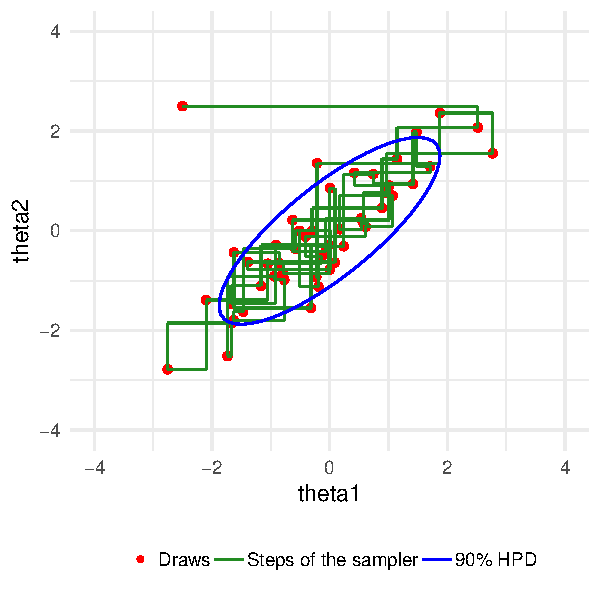
\includegraphics[width=5cm]{Gibbs1.pdf}
     \end{center}
    \vspace{-.5\baselineskip}
     \item<3-> Basic algorithm {
      \begin{align*}
         \text{sample $\theta_j^t$ from} \quad & p(\theta_j|\theta_{-j}^{t-1}, y),\\
      \text{where} \quad
        & \theta^{t-1}_{-j}= (\theta^t_1,\dots,\theta^t_{j-1},
        \theta^{t-1}_{j+1},\dots,\theta^{t-1}_d)
      \end{align*}
      }
  \end{itemize}

\end{frame}

\begin{frame}

  {\Large\color{navyblue} Gibbs sampling}

  \vspace{-0.5\baselineskip}
  \begin{itemize}
  \item With {\it conditionally} conjugate priors, the sampling from
    the conditional distributions is easy for wide range of models
    \begin{itemize}
      \item BUGS/WinBUGS/OpenBUGS/JAGS
    \end{itemize}
  \item<2-> No algorithm parameters to tune\\
    (cf. proposal distribution in Metropolis algorithm)
  \item<3-> For not so easy conditionals, use  e.g. inverse-CDF
  \item<4-> Several parameters can be updated in blocks ({\em blocking})
  \item<5-> Slow if parameters are highly dependent in the posterior
    \begin{itemize}
    \item<5-> demo11\_1 continues\\
      \vspace{-0.5\baselineskip}
      \hspace{3.5cm}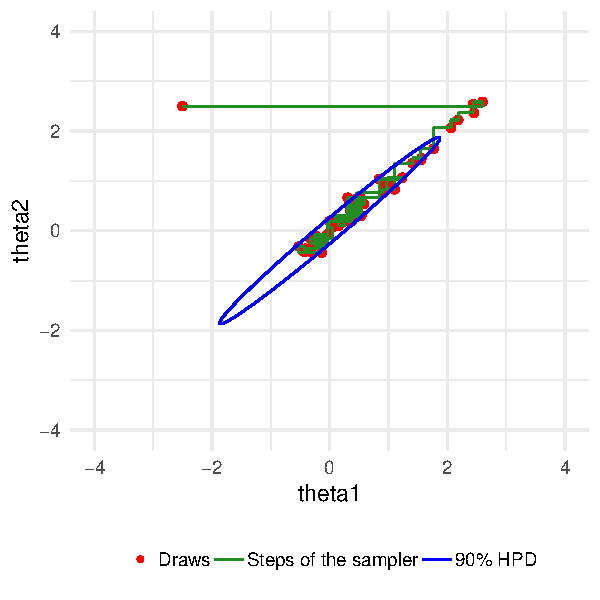
\includegraphics[width=5cm]{Gibbs2.pdf}
    \end{itemize}
  \end{itemize}

\end{frame}

\begin{frame}

  {\Large\color{navyblue} Conditional vs joint}

  \begin{itemize}
  \item How about sampling $\theta$ jointly?
    \begin{itemize}
    \item e.g. it is easy to sample from multivariate normal
    \end{itemize}
    \item<2-> Can we use that to form a Markov chain?\\
      {\small \url{http://elevanth.org/blog/2017/11/28/build-a-better-markov-chain/}}
  \end{itemize}

\end{frame}

\begin{frame}

  {\Large\color{navyblue} Metropolis algorithm}

  \begin{itemize}
  \item Algorithm
    \begin{itemize}
      \item[1.] starting point $\theta^0$
      \item[2.] $t=1,2,\ldots$
        \begin{itemize}
        \item[(a)] pick a proposal $\theta^{*}$ from the proposal distribution
          $J_t(\theta^{*}|\theta^{t-1})$. \\
          Proposal distribution has to be symmetric, i.e.\\
          $J_t(\theta_a|\theta_b)=J_t(\theta_b|\theta_a)$, for all
          $\theta_a,\theta_b$
        \item<2->[(b)] calculate acceptance ratio
          \begin{equation*}
            r=\frac{p(\theta^{*}|y)}{p(\theta^{t-1}|y)}
          \end{equation*}
          \vspace{-6mm}
        \item<3->[(c)] set
          \begin{equation*}
            \theta^t=
            \begin{cases}
              \theta^{*} & \text{with probability $\min(r,1)$}\\
              \theta^{t-1} & \text{otherwise}
            \end{cases}
          \end{equation*}
          \uncover<4>{
          ie, if $p(\theta^{*}|y)>p(\theta^{t-1})$ accept the proposal always \\
          \hspace{0.4cm}and otherwise reject the proposal with probability $r$}
      \end{itemize}
      \vspace{-1.5\baselineskip}
    \item<5-> rejection of a proposal increments the time $t$ also by one\\
      ie, the new state is the same as previous
      \item<6-> step c is executed by generating a random number from 
        $\U(0,1)$
      \item<7-> instead of $p(\theta|y)$, unnormalized $q(\theta|y)$ can be used,
        as the normalization terms cancel out!
      \vspace{-0mm}
    \end{itemize}
  \end{itemize}

\end{frame}

\begin{frame}

  {\Large\color{navyblue} Metropolis algorithm}

  \begin{itemize}
  \item Example: one bivariate observation $(y_1,y_2)$
    \begin{itemize}
    \item bivariate normal distribution with unknown mean and known
      covariance
       \begin{equation*}
         \left.
         \begin{pmatrix}
           \theta_1\\
           \theta_2
         \end{pmatrix}
         \right| y \sim
         \N\left(
           \begin{pmatrix}
             y_1\\
             y_2
           \end{pmatrix},
           \begin{pmatrix}
             1 & \rho\\
             \rho & 1
         \end{pmatrix}
       \right)
       \end{equation*}
     \item proposal distribution
       $J_t(\theta^{*}|\theta^{t-1})=\N(\theta^{*}|\theta^{t-1},\sigma_p^2)$
     \end{itemize}
   \item Demo {\small \url{http://elevanth.org/blog/2017/11/28/build-a-better-markov-chain/}}
   \end{itemize}

\end{frame}

 \begin{frame}

  {\Large\color{navyblue} Why Metropolis algorithm works}

  \begin{itemize}
  \item Intuitively more draws from the higher density areas as
    jumps to higher density are always accepted and only some of the
    jumps to the lower density are accepted
    \vspace{5mm}
    \pause
  \item Theoretically
    \begin{itemize}
    \item[1.] Prove that simulated series is a Markov chain
      which has unique stationary distribution
    \item[2.] Prove that this stationary distribution is the desired target distribution
    \end{itemize}
\end{itemize}

\end{frame}

\begin{frame}
  
  {\Large\color{navyblue} Why Metropolis algorithm works}
  
  \begin{itemize}
  \item[1.] Prove that simulated series is a Markov chain
    which has unique stationary distribution
    \begin{itemize}
    \item[a)] irreducible
      \begin{itemize}
      \item<2->[=] positive probability of eventually reaching any
        state from any other state
      \end{itemize}
    \item[b)] aperiodic
      \begin{itemize}
      \item<3->[=] aperiodic (return times are not periodic)
      \item<3->[-] holds for a random walk on any proper distrbution (except for trivial exceptions)
      \end{itemize}
    \item[c)] recurrent / not transient
      \begin{itemize}
      \item<4->[=] probability to return to a state $i$ is 1
      \item<4->[-] holds for a random walk on any proper distrbution (except for trivial exceptions)
      \end{itemize}
    \end{itemize}
  \end{itemize}
  
\end{frame}

\begin{frame}
  
  {\Large\color{navyblue} Why Metropolis algorithm works}

  \begin{itemize}
  \item[2.] Prove that this stationary distribution is the desired target distribution $p(\theta|y)$
    \begin{itemize}
    \item[-] consider starting algorithm at time $t-1$ with a draw
      $\theta^{t-1} \sim p(\theta|y)$ 
    \item<2->[-] consider any two such points $\theta_a$ ja $\theta_b$ drawn
      from $p(\theta|y)$ and labeled so that
      $p(\theta_b|y)\geq p(\theta_a|y)$
    \item<3->[-] the unconditional probability density of a transition from $\theta_a$ to $\theta_b$ is
      \vspace{-0.5\baselineskip}
      \begin{equation*}
        p(\theta^{t-1}=\theta_a,\theta^{t}=\theta_b)=
        p(\theta_a|y)J_t(\theta_b|\theta_a),
      \end{equation*}
      \vspace{-1\baselineskip}
    \item<4->[-] the unconditional probability density of a transition from $\theta_b$ to $\theta_a$ is
      \vspace{-0.5\baselineskip}
      \begin{eqnarray*}
        p(\theta^{t}=\theta_a,\theta^{t-1}=\theta_b) & = &
        p(\theta_b|y)J_t(\theta_a|\theta_b)\left(\frac{p(\theta_a|y)}{p(\theta_b|y)}\right)\\
        \pause &  = &  p(\theta_a|y)J_t(\theta_a|\theta_b),
      \end{eqnarray*}
      \uncover<5->{
      which is the same as the probability of transition from $\theta_a$ to $\theta_b$,
      since we have required that $J_t(\cdot|\cdot)$ is symmetric}
      \pause
    \item<6->[-] since their joint distribution is symmetric, $\theta^t$ and
      $\theta^{t-1}$ have the same marginal distributions, and so
      $p(\theta|y)$ is the stationary distribution of the Markov chain of $\theta$
    \end{itemize}
  \end{itemize}

\end{frame}

\begin{frame}

  {\Large\color{navyblue} Metropolis-Hastings algorithm}

  \begin{itemize}
  \item Generalization of Metropolis algorithm for non-symmetric proposal distributions
    \begin{itemize}
    \item acceptance ratio includes ratio of proposal distributions
      \begin{equation*}
        r =
        \frac{p(\theta^{*}|y)/J_t(\theta^{*}|\theta^{t-1})}{p(\theta^{t-1}|y)/J_t(\theta^{t-1}|\theta^{*})} \pause =
        \frac{p(\theta^{*}|y)J_t(\theta^{t-1}|\theta^{*})}{p(\theta^{t-1}|y)J_t(\theta^{*}|\theta^{t-1})}
      \end{equation*}
    \end{itemize}
  \end{itemize}

\end{frame}

% \begin{frame}

%   {\Large\color{navyblue} Metropolis-Hastings algorithm}

%   \begin{itemize}
%   \item More efficient proposal distributions
%     \item e.g. Langevin-Hastings algorithm which uses gradient information to make proposals
%         \begin{itemize}
%         \item more likely to propose values with higher density
%         \end{itemize}
%   \end{itemize}

% \end{frame}

\begin{frame}

  {\Large\color{navyblue} Metropolis-Hastings algorithm}

  \begin{itemize}
  \item Ideal proposal distribution is the distribution itself
    \begin{itemize}
    \item $J(\theta^{*}|\theta)\equiv p(\theta^{*}|y)$ for all
      $\theta$
    \item acceptance probability is $1$
    \item independent draws
    \item not usually feasible
    \end{itemize}
  \item<2-> Good proposal distribution resembles the target distribution
    \begin{itemize}
    \item if the shape of the target distribution is unknown, usually
      normal or $t$ distribution is used
    \end{itemize}
  \item<3-> After the shape has been selected, it is important to select the scale
    \begin{itemize}
    \item small scale \\$\rightarrow$ many steps accepted, but the chain moves slowly due to small steps
    \item big scale \\$\rightarrow$ long steps proposed, but many of
      those rejected and again chain moves slowly
    \end{itemize}
  \item<4-> Generic rule for rejection rate is 60-90\% (but depends on
    dimensionality and a specific algorithm variation)
\end{itemize}

\end{frame}

% \begin{frame}

%   {\Large\color{navyblue} Metropolis-Hastings algorithm}

%   \begin{itemize}
%   \item Update of parameters
%     \begin{itemize}
%     \item jointly
%     \item blocked
%     \item  single-component
%     \end{itemize}
%   \item Order of single or blocked updates is free
%     \begin{itemize}
%       \item same for all rounds
%       \item random
%       \item not all parameters updated each round
%     \end{itemize}
%   \end{itemize}

% \end{frame}

\begin{frame}

  {\Large\color{navyblue} Gibbs sampling}

  \begin{itemize}
  \item Specific case of Metropolis-Hastings algorithm
    \begin{itemize}
    \item single updated (or blocked)
    \item proposal distribution is the conditional distribution\\
      $\rightarrow$ proposal and target distributions are same\\
      $\rightarrow$ acceptance probability is $1$
    \end{itemize}
  \end{itemize}  

\end{frame}

\begin{frame}

  {\Large\color{navyblue} Metropolis}

  \begin{itemize}
  \item Ususally doesn't scale well to high dimensions
    \begin{itemize}
    \item if the shape doesn't match the whole distribution, the efficiency drops
    \item demo11\_2\\
      \vspace{1\baselineskip}
      \hspace{-1cm}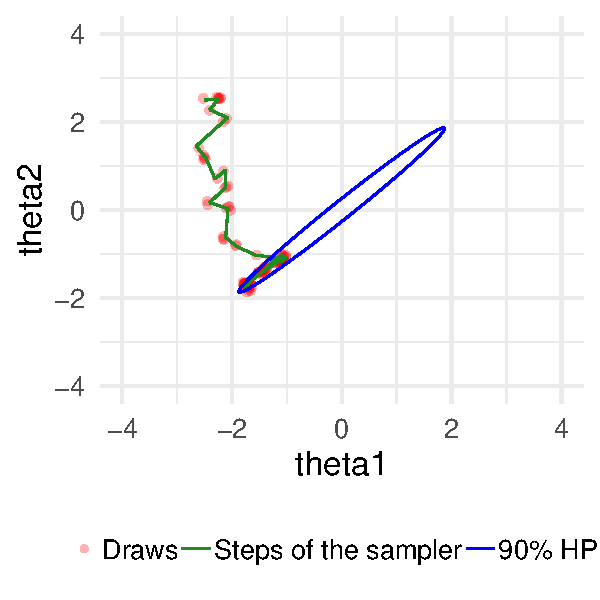
\includegraphics[width=5cm]{Metrop2.pdf}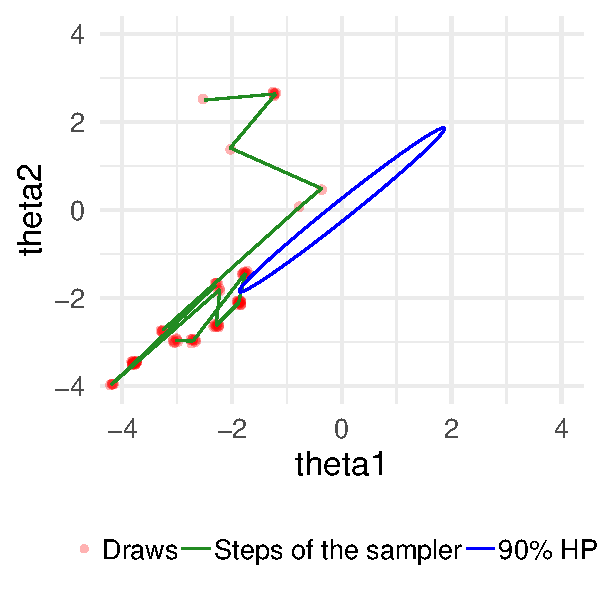
\includegraphics[width=5cm]{Metrop3.pdf}
    \end{itemize}
  \end{itemize}  

\end{frame}


\begin{frame}

  {\Large\color{navyblue} Dynamic Hamiltonian Monte Carlo and NUTS}

  \begin{itemize}
  \item Chapter 12 presents some more advanced methods
    \begin{itemize}
    \item Chapter 12 includes Hamiltonian Monte Carlo and NUTS, which
      is one of the most efficient methods
      \begin{itemize}
      \item uses gradient information
      \item Hamiltonian dynamic simulation reduces random walk
   \item Demo {\small \url{http://elevanth.org/blog/2017/11/28/build-a-better-markov-chain/}}
      \end{itemize}
    \end{itemize}
  \end{itemize}  

\end{frame}

\begin{frame}

  {\Large\color{navyblue} HMC / NUTS}

  \vspace{-.5\baselineskip}
  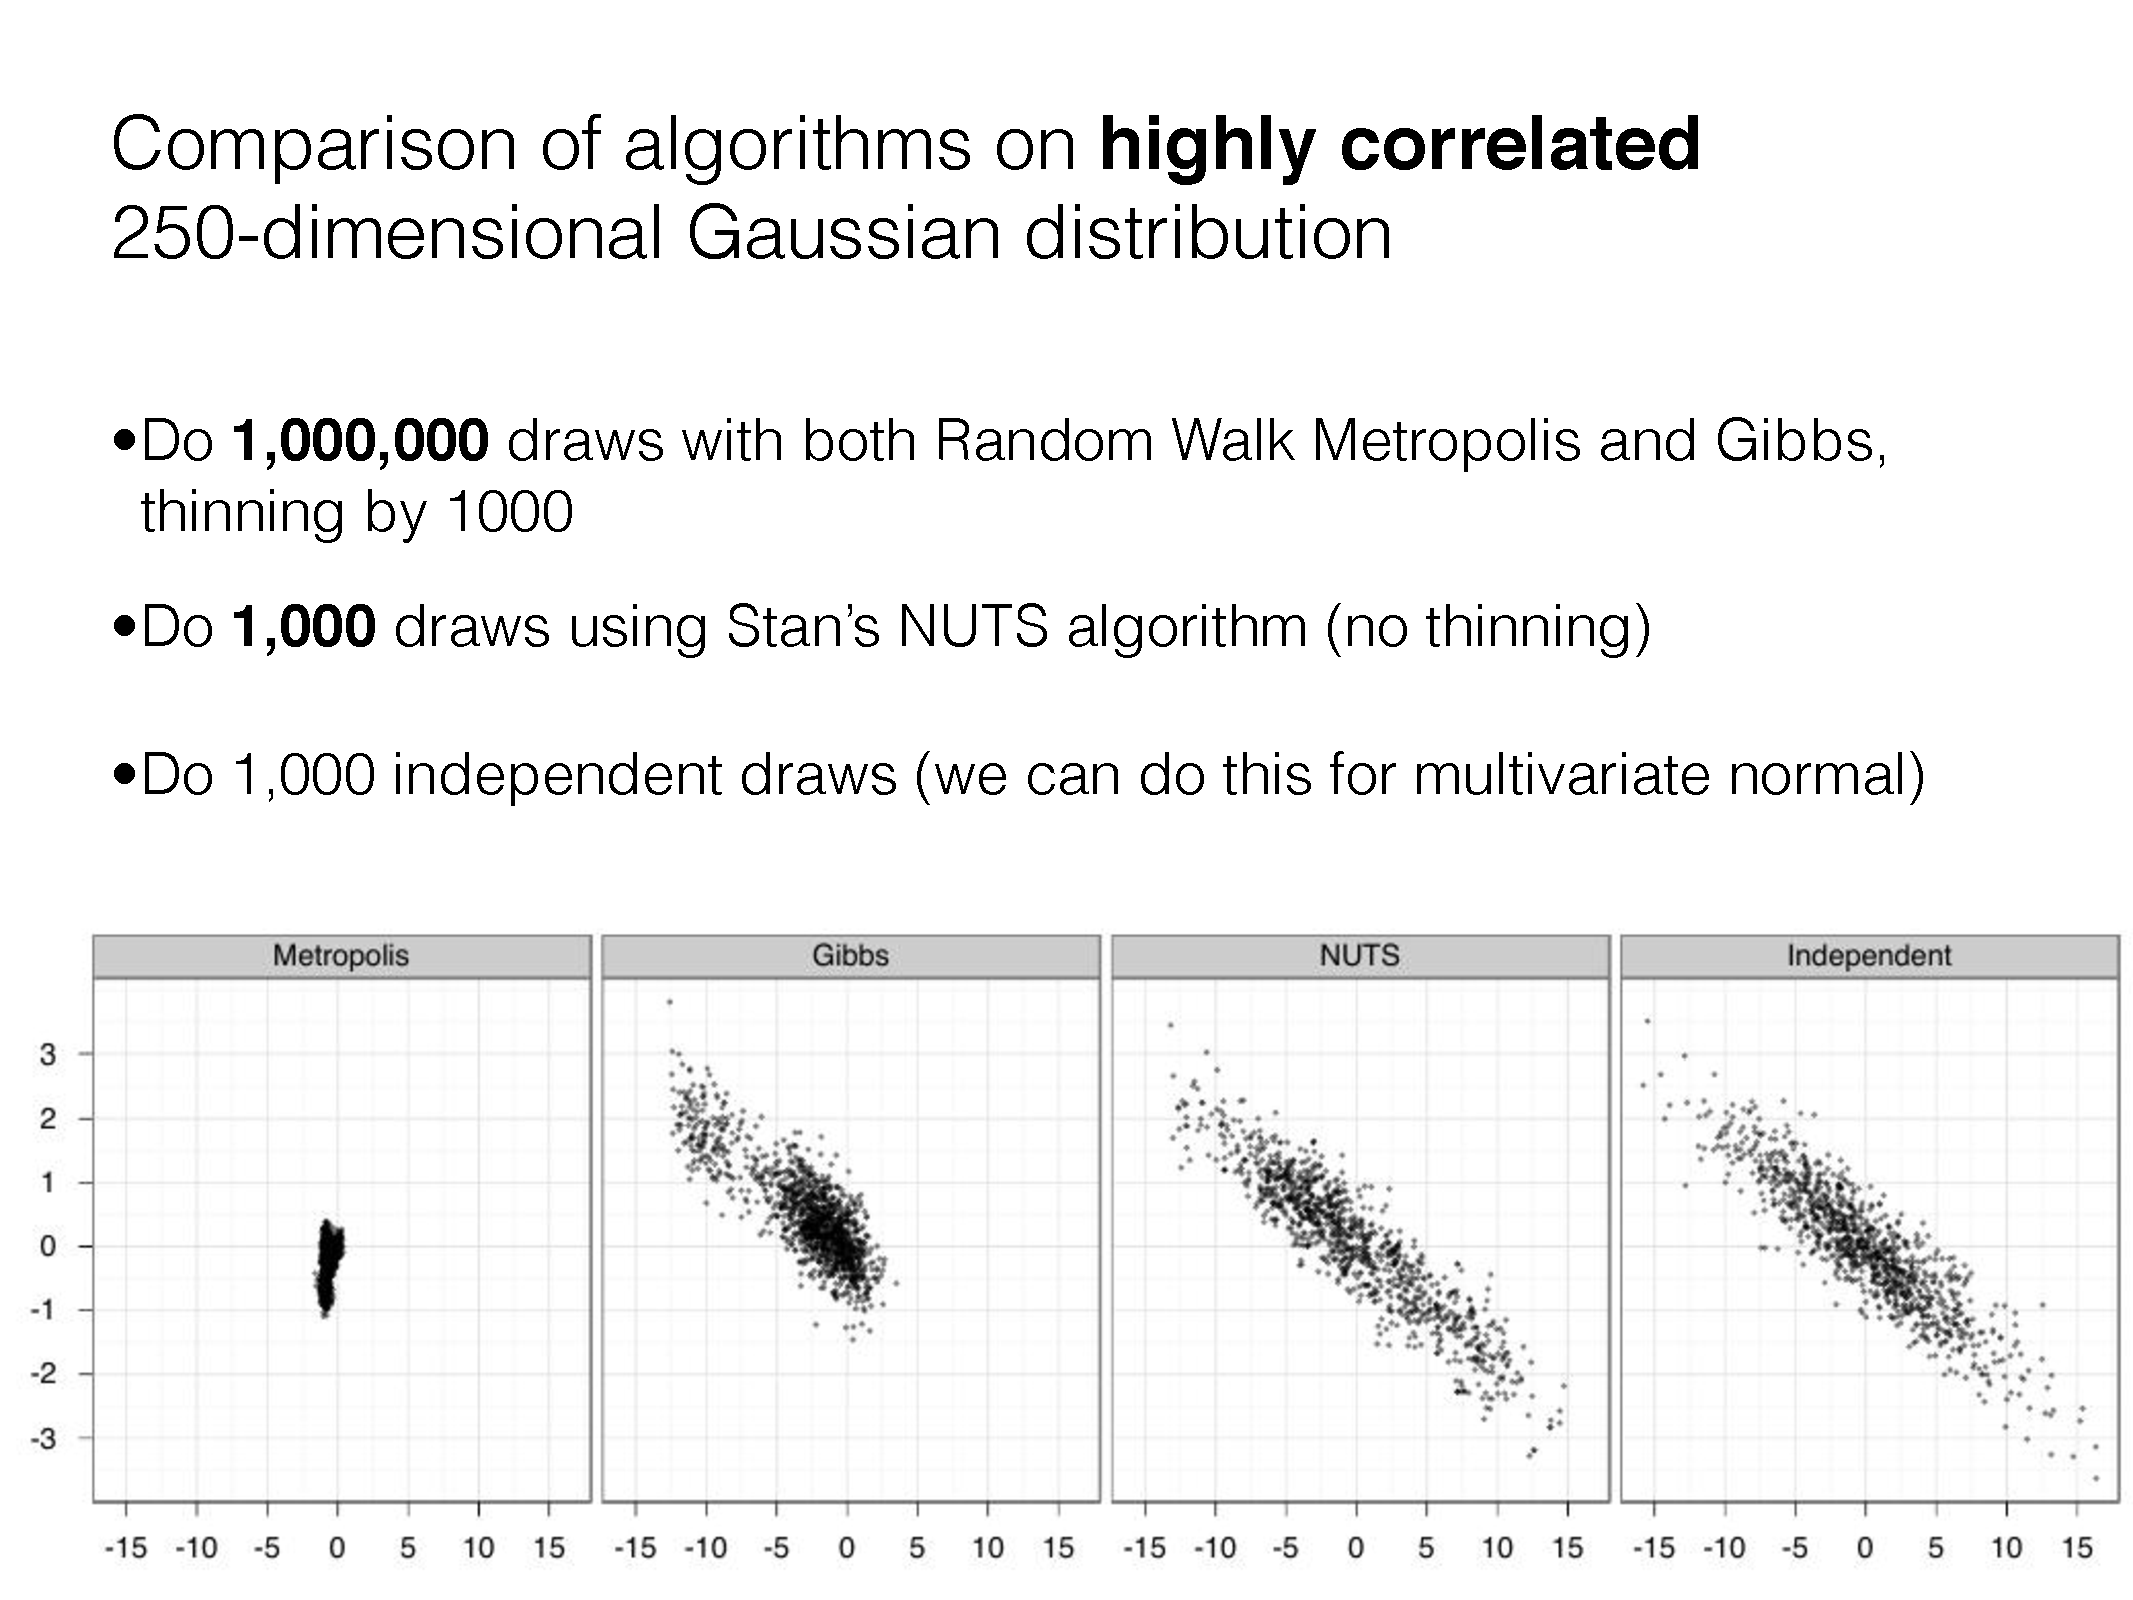
\includegraphics[width=\textwidth,clip]{N250.pdf}\\
  Source: Jonah Gabry

\end{frame}

% \begin{frame}{HMC / NUTS}
%   \includegraphics[width=\textwidth,clip]{typicalset49.pdf}
% \end{frame}

% \begin{frame}{HMC / NUTS}
%   \includegraphics[width=\textwidth,clip]{typicalset50.pdf}
% \end{frame}

% \begin{frame}{HMC / NUTS}
%   \includegraphics[width=\textwidth,clip]{typicalset51.pdf}
% \end{frame}

% \begin{frame}{HMC / NUTS}
%   \includegraphics[width=\textwidth,clip]{typicalset52.pdf}
% \end{frame}

% \begin{frame}{Hamiltonian Monte Carlo}

%   \begin{itemize}
%   \item demo12\_1
%   \item Uses gradient information for more efficient sampling
%   \item Alternating dynamic simulation and sampling of the energy
%     level
%   \item Parameters
%     \begin{itemize}
%     \item step size, number of steps in each chain
%     \end{itemize}
% \pause
% \item No U-Turn Sampling
%   \begin{itemize}
%   \item adaptively selects number of steps to improve robustness and
%     efficiency
%   \end{itemize}
% \pause
% \item Adaptation in Stan
%   \begin{itemize}
%   \item Step size adjustment (mass matrix) is estimated during initial
%     adaptation phase
%   \end{itemize}
% \item See more
%   \begin{itemize}
%   \item \url{https://icerm.brown.edu/video_archive/\#/play/1107}
%   \item \url{https://arxiv.org/abs/1701.02434}
%   \end{itemize}
% \end{itemize}

% \end{frame}

\begin{frame}

  {\Large\color{navyblue} Warm-up and convergence diagnostics}

  \begin{itemize}
  \item Asymptotically chain spends the $\alpha$\% of time where
    $\alpha$\% posterior mass is
    \uncover<2->{
      \begin{itemize}
      \item but in finite time the initial part of the chain may be
        non-representative and lower error of the estimate can be
        obtained by throwing it away\\
        \hspace{2cm}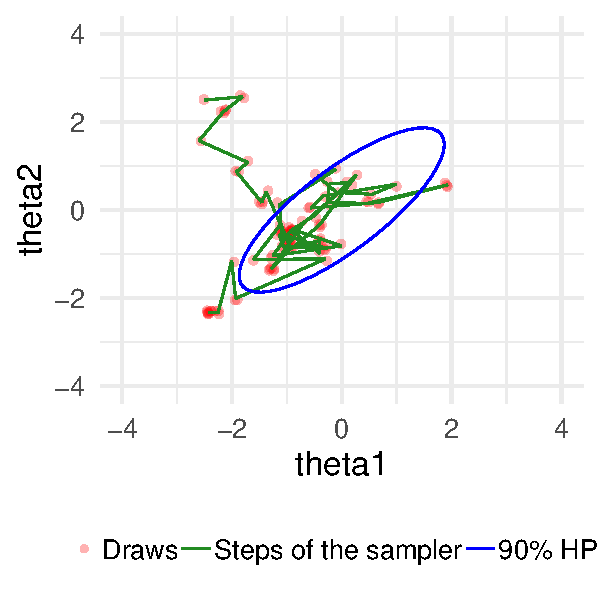
\includegraphics[width=4cm]{Metrop1.pdf}
      \end{itemize}
      }
      \vspace{-.5\baselineskip}
    \item<3-> Warm-up = remove draws from the beginning of the chain
      \begin{itemize}
      \item warm-up may include also phase for adapting algorithm parameters
      \end{itemize}
    \item<4-> Convergence diagnostics 
      \begin{itemize}
      \item Do we get samples from the target distribution?
      \end{itemize}
  \end{itemize}

\end{frame}

\begin{frame}

  {\Large\color{navyblue} MCMC draws are dependent}

  \begin{itemize}
    \item Monte Carlo estimates still valid (central limit theorem holds)
      \begin{align*}
        E_{\color{blue} p(\theta|y)}[f(\theta)] \approx \frac{1}{S} \sum_{s=1}^S f(\theta^{(s)})
      \end{align*}
    \item Estimation of Monte Carlo error is more difficult
      \begin{itemize}
      \item evaluation of {\it effective} sample size
      \end{itemize}
    \end{itemize}  

\end{frame}

\begin{frame}

  {\Large\color{navyblue} Several chains}

  \vspace{-0.5\baselineskip}
  \begin{itemize}
  \item Use of several chains make convergence diagnostics easier
    \item Start chains from different starting points -- preferably overdispersed
      \begin{center}
  \vspace{-0.5\baselineskip}
      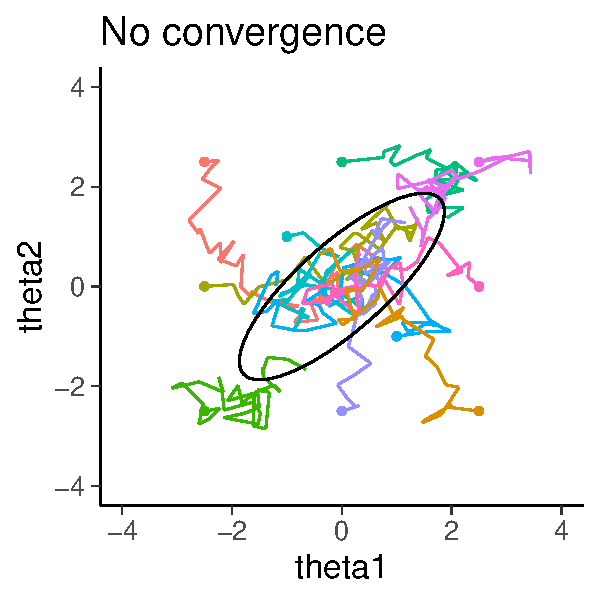
\includegraphics[width=6cm]{10chains1.pdf}
    \end{center}
  \vspace{-0.5\baselineskip}
    \item<2-> Remove draws from the beginning of the chains and run
      chains long enough so that it is not possible to distinguish
      where each chain started and the chains are well mixed
  \end{itemize}

\end{frame}

\begin{frame}

  {\Large\color{navyblue} Several chains}

      \begin{center}
      \only<1>{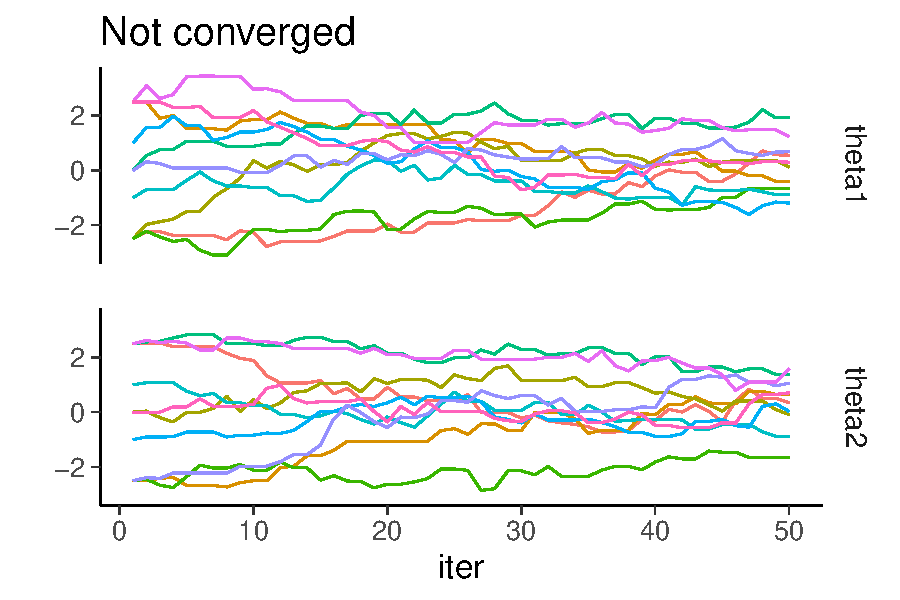
\includegraphics[width=10cm]{10chains2.pdf}}
      \only<2->{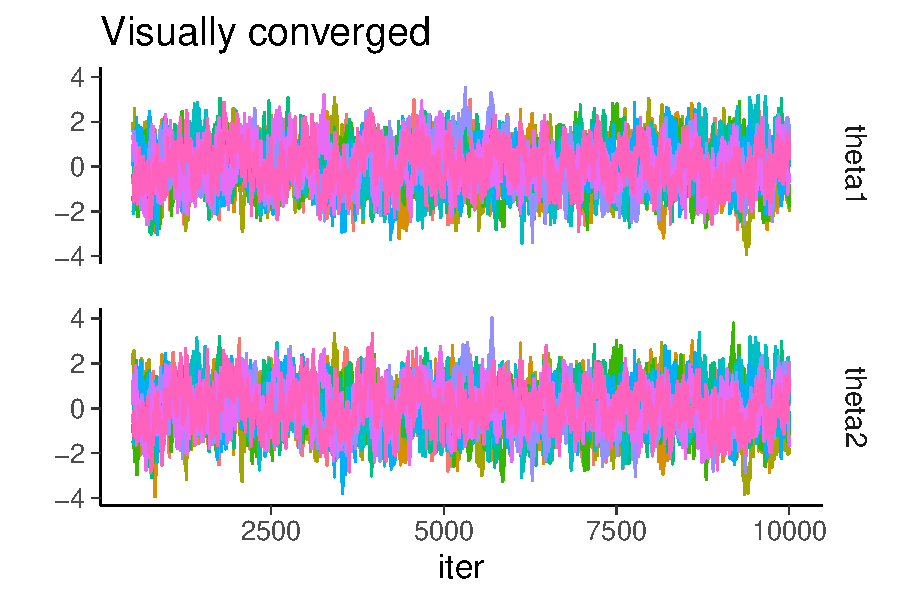
\includegraphics[width=10cm]{10chains3.pdf}}\\
      \uncover<3->{Visual convergence check is not sufficient}
    \end{center}

\end{frame}

\begin{frame}[fragile]

  {\Large\color{navyblue} $\widehat{R}$: comparison of within and between variances of the chains}

  \begin{itemize}
  \item BDA3: $\widehat{R}$ aka {\em potential scale reduction factor} (PSRF)
  \item Compare means and variances of the chains\\
    \uncover<2->{W = within chain variance estimate\\
    var\_hat\_plus = total variance estimate\\}
    \vspace{1\baselineskip}
    \only<1>{\hspace{-0.5cm}\phantom{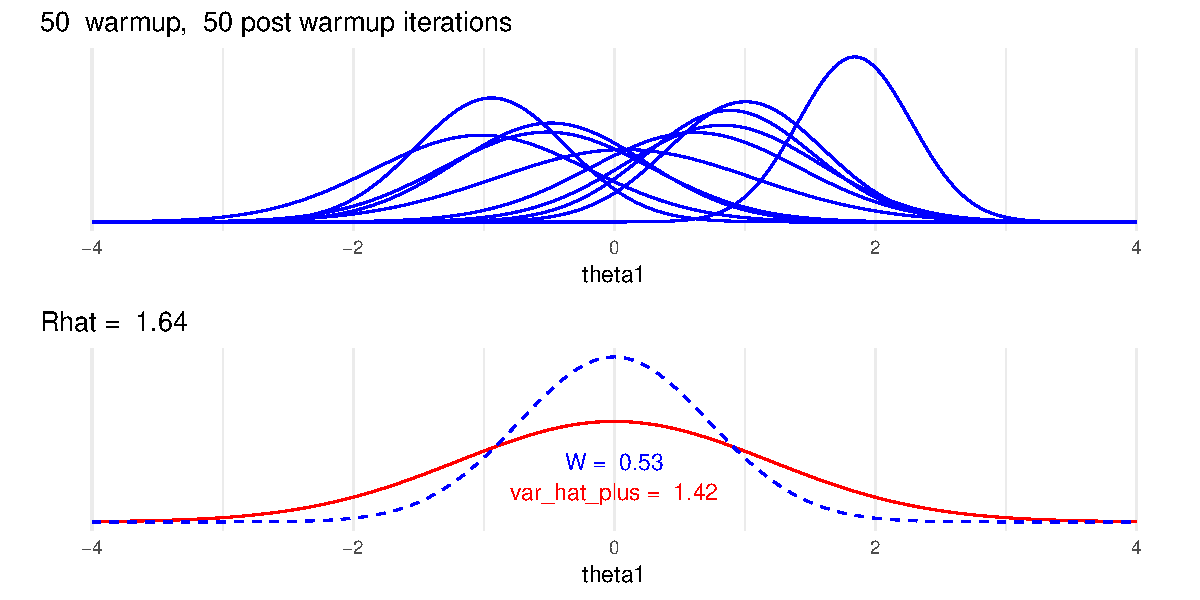
\includegraphics[width=10.5cm]{10chains_rhat1.pdf}}}
    \only<2>{\hspace{-0.5cm}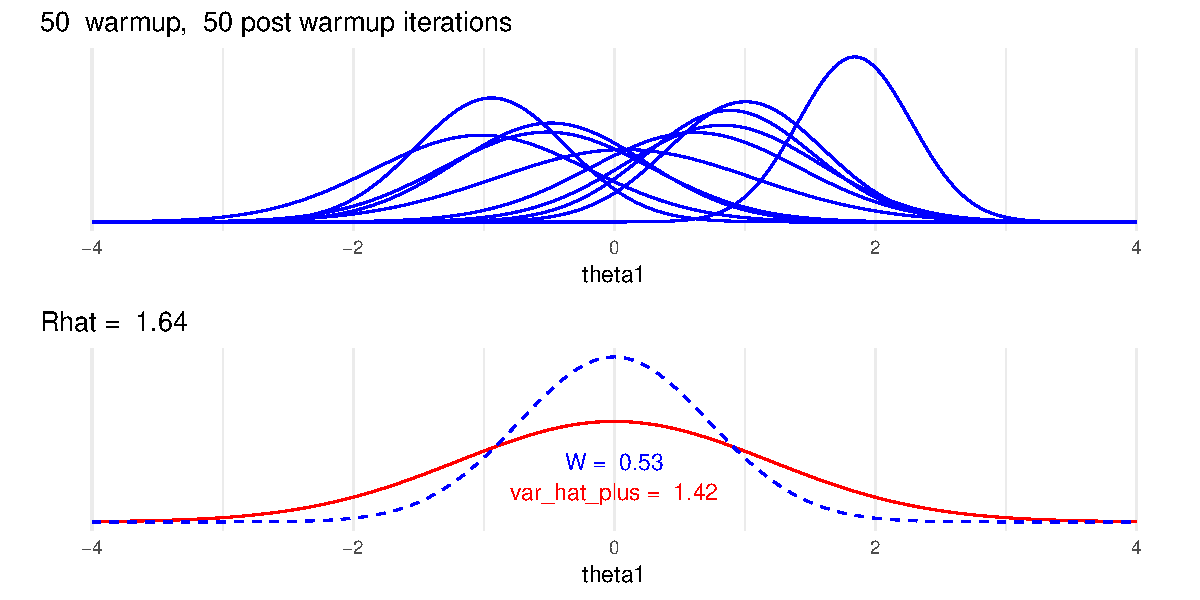
\includegraphics[width=10.5cm]{10chains_rhat1.pdf}}
    \only<3>{\hspace{-0.5cm}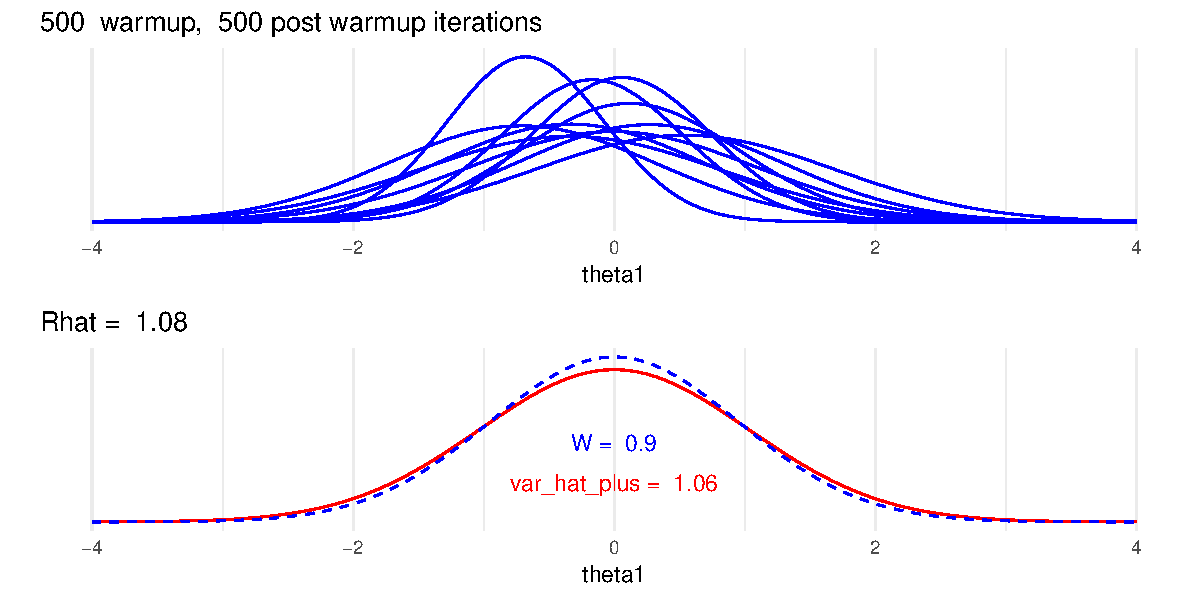
\includegraphics[width=10.5cm]{10chains_rhat2.pdf}}
    \only<4>{\hspace{-0.5cm}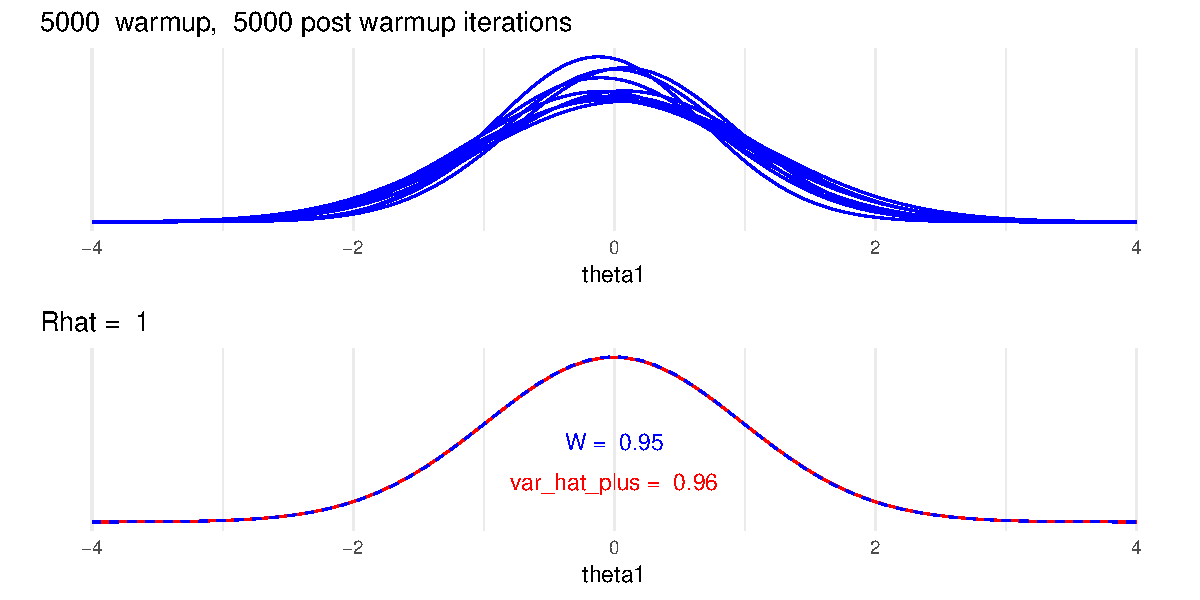
\includegraphics[width=10.5cm]{10chains_rhat3.pdf}}
  \end{itemize}  

\end{frame}

\begin{frame}
  
  {\Large\color{navyblue} $\widehat{R}$}

  \begin{itemize}
  \item<1-> Within chains variance $W$
    \begin{equation*}
      W=\frac{1}{m}\sum_{j=1}^m s^2_j ,\text{ where } 
      s^2_j=\frac{1}{n-1}\sum_{i=1}^n (\psi_{ij}-\bar{\psi}_{.j})^2
    \end{equation*}
  \item<2-> Between chains variance $B$
    \begin{equation*}
      B=\frac{n}{m-1}\sum_{j=1}^m
      (\bar{\psi}_{.j}-\bar{\psi}_{..})^2,
      \text{ where } \bar{\psi}_{.j}=\frac{1}{n}\sum_{i=1}^n \psi_{ij},
      \bar{\psi}_{..}=\frac{1}{m}\sum_{j=1}^m\bar{\psi}_{.j}
    \end{equation*}
    \vspace{-6mm}
    \begin{itemize}
      \item $B/n$ is variance of the means of the chains
    \end{itemize}
    \vspace{2mm}
  \item<3-> Estimate total variance
    $\var(\psi|y)$ as a weighted mean of $W$ and $B$
    \begin{equation*}
      \widehat{\var}^{+}(\psi|y) = \frac{n-1}{n}W+\frac{1}{n}B
    \end{equation*}
  \end{itemize}  

\end{frame}

% \note{1) $B/n$ on varsinainen ketjujen keskiarvojen varianssi, jossa $n$
% johtuu siit� ett� ne keskiarvot joiden varianssia lasketaan on
% muodostettu $n$ n�ytteest� ja siten varianssi pienempi, mutta
% Gelman et kump. ovat halunneet merkit� kuitenkin $B$:ll� $n$ kertaa
% t�t� varianssia, koska silloin lopullisessa
% marginaaliposteriorivarianssin kaavassa n�kyy $n$:n vaikutus

% 2) termi $\frac{n-1}{n}$ tulee siit�, ett� silloin painojen summa on 1
% }

\begin{frame}

  {\Large\color{navyblue} $\widehat{R}$}

  \begin{itemize}
  \item Estimate total variance
    $\var(\psi|y)$ as a weighted mean of $W$ and $B$
    \begin{equation*}
      \widehat{\var}^{+}(\psi|y) = \frac{n-1}{n}W+\frac{1}{n}B
    \end{equation*}
    \vspace{-0.5\baselineskip}
    \begin{itemize}
    \item this \emph{overestimates} marginal posterior variance if the
      starting points are overdispersed
    \end{itemize}
    \vspace{0.5\baselineskip}
  \item<2-> Given finite $n$, $W$ \emph{underestimates} marginal posterior variance
    \begin{itemize}
    \item single chains have not yet visited all points in the distribution
    \item when $n\rightarrow\infty, \quad \E(W)\rightarrow \var(\psi|y)$
    \end{itemize}
    \vspace{0.5\baselineskip}
  \item<3-> As $\widehat{\var}^{+}(\psi|y)$ overestimates and $W$ underestimates,
    compute
    \begin{equation*}
      \widehat{R}=\sqrt{\frac{\widehat{\var}^{+}}{W}}
    \end{equation*}
\end{itemize}  

\end{frame}

\begin{frame}[fragile]

  {\Large\color{navyblue} $\widehat{R}$}

  \begin{itemize}
  \item BDA3: $\widehat{R}$ aka {\em potential scale reduction factor} (PSRF)
  \item Compare means and variances of the chains\\
    W = within chain variance estimate\\
    var\_hat\_plus = total variance estimate\\
    \vspace{1\baselineskip}
    \only<1>{\hspace{-0.5cm}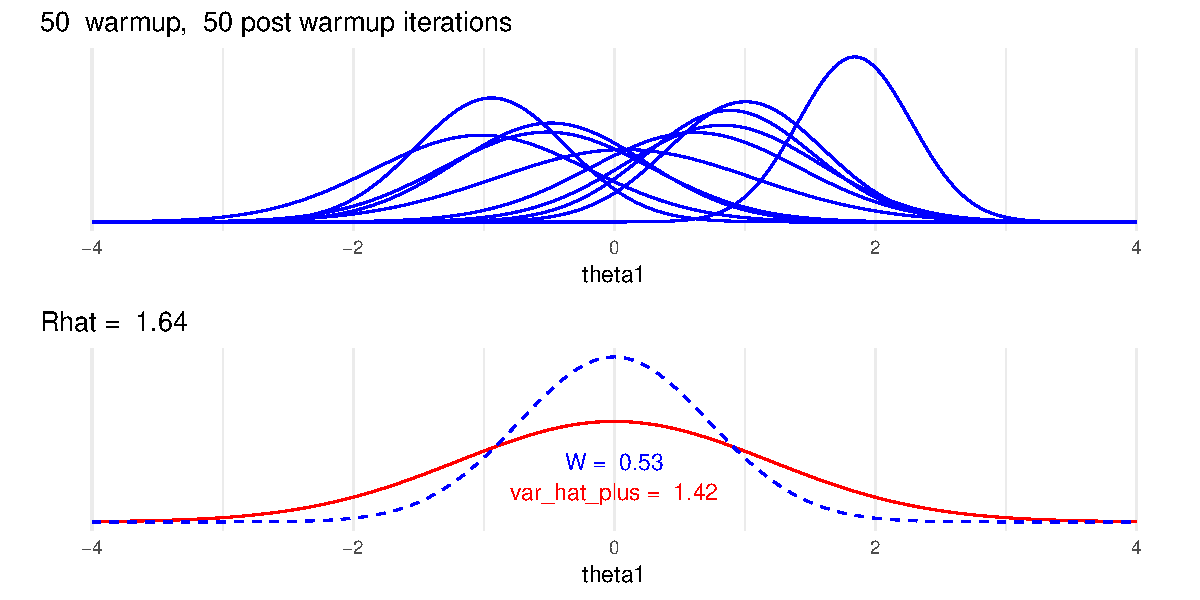
\includegraphics[width=10.5cm]{10chains_rhat1.pdf}}
    \only<2>{\hspace{-0.5cm}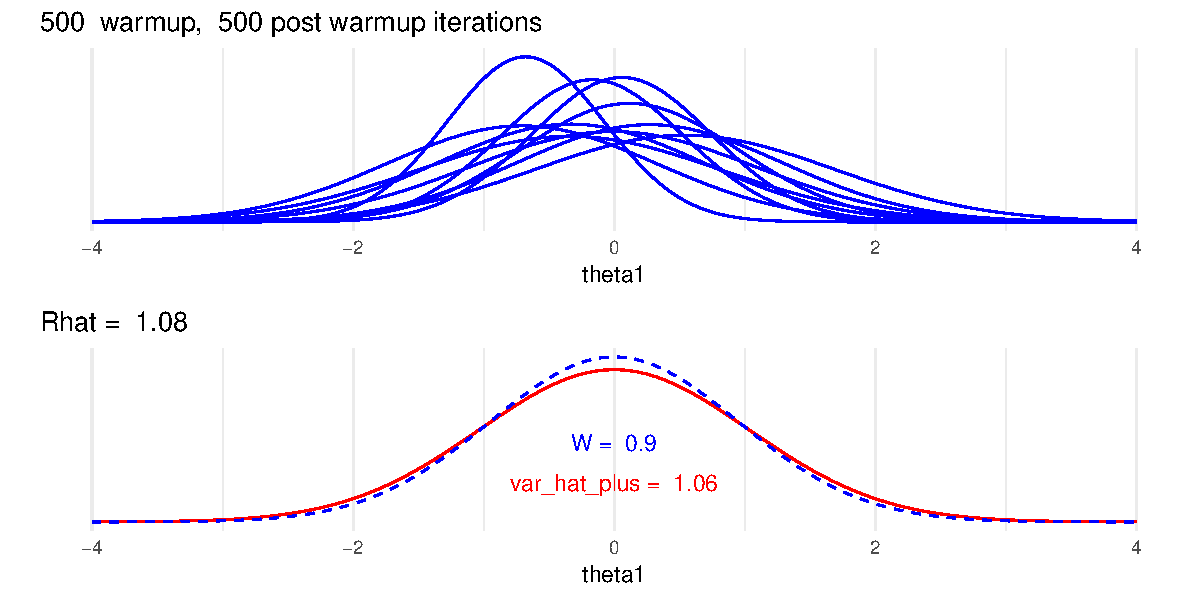
\includegraphics[width=10.5cm]{10chains_rhat2.pdf}}
    \only<3>{\hspace{-0.5cm}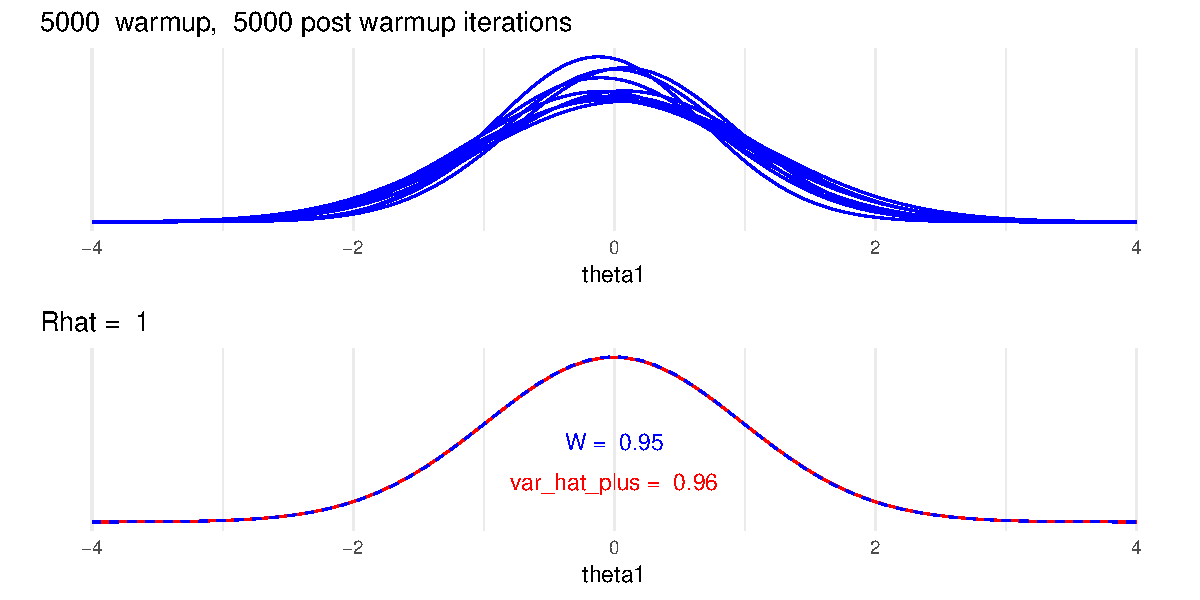
\includegraphics[width=10.5cm]{10chains_rhat3.pdf}}
  \end{itemize}  

\end{frame}

\begin{frame}

  {\Large\color{navyblue} $\widehat{R}$}

  \begin{equation*}
      \widehat{R}=\sqrt{\frac{\widehat{\var}^{+}}{W}}
    \end{equation*}
    \begin{itemize}
    \item<1-> Estimates how much the scale of $\psi$ could reduce if $n\rightarrow\infty$
    \item<1-> $R\rightarrow 1$, when $n\rightarrow\infty$
    \item<1-> if $R$ is big (e.g., $R>1.01$), keep sampling
    \item<2-> If $R$ close to 1, it is still possible that chains have not converged
      \begin{itemize}
      \item if starting points were not overdispersed
      \item distribution far from normal (especially if infinite variance)
      \item just by chance when $n$ is finite
      \end{itemize}
    \end{itemize}  

\end{frame}

\begin{frame}[fragile]

  {\Large\color{navyblue} Split-$\widehat{R}$}

  \begin{itemize}
  \item BDA3: split-$\widehat{R}$
  \item Examines {\it mixing} and {\it stationarity} of chains
  \item To examine stationarity chains are splitted to two parts
    \begin{itemize}
    \item after splitting, we have $m$ chains, each having $n$ draws
    \item scalar draws $\psi_{ij} \quad (i=1,\ldots,n;j=1,\ldots,m)$
    \item compare means and variances of the split chains
    \end{itemize}
  \end{itemize}  

\end{frame}


% \begin{frame}
  
%   {\Large\color{navyblue} Convergence diagnostics}

%   \begin{itemize}
%   \item After how many iterations can we check for convergence
%     \begin{itemize}
%     \item it's not possible to no this beforehand
%     \item Stan uses NUTS which is an efficient sampler and default is
%       to use 4 chains, get 1000 draws from each for adaptation and
%       warmup, 1000 more draws from each and estimate $\widehat{R}$ for
%       each parameter
%     \end{itemize}
%   \end{itemize}

% \end{frame}

% \begin{frame}{Divergences}

%   \begin{itemize}
%   \item Diagnosing difficult to reach corners of the posterior
%   \item Case study \url{http://mc-stan.org/users/documentation/case-studies/divergences_and_bias.html}
%   \end{itemize}

% \end{frame}

% \begin{frame}{Tree depth}

%   \begin{itemize}
%   \item Diagnosing long tails
%   \item Case studies
%     \begin{itemize}
%     \item R: \url{http://mc-stan.org/users/documentation/case-studies/rstan_workflow.html}
%     \item Python: \url{http://mc-stan.org/users/documentation/case-studies/pystan_workflow.html}
%     \end{itemize}
    
%   \end{itemize}

% \end{frame}

\begin{frame}

  {\Large\color{navyblue} Time series analysis}

  \begin{itemize}
  \item Auto correlation function
    \begin{itemize}
    \item describes the correlation given a certain lag
    \item can be used to compare efficiency of MCMC algorithms and parameterizations
    \end{itemize}
  \end{itemize}
% \vspace{.5cm}
%   \begin{center}
%       \includegraphics[scale=.8,clip]{kuva11_1}
%   \end{center}
\end{frame}

\begin{frame}

  {\Large\color{navyblue} Auto correlation}

  \vspace{-0.5\baselineskip}
  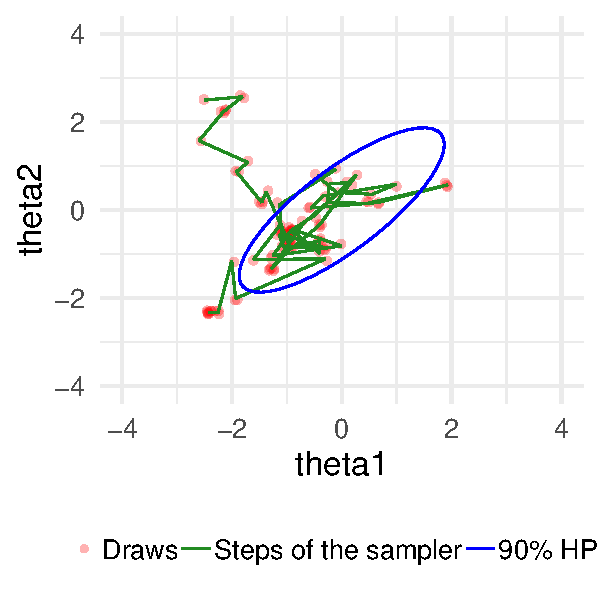
\includegraphics[width=4.5cm]{Metrop1.pdf}
  \uncover<2->{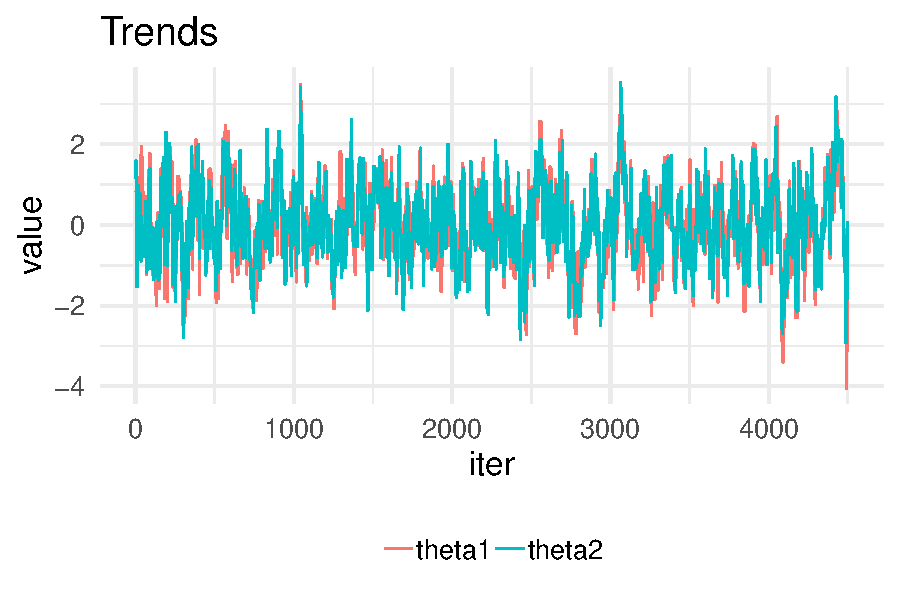
\includegraphics[width=7cm]{Metrop1trace.pdf}\\}
  \uncover<3->{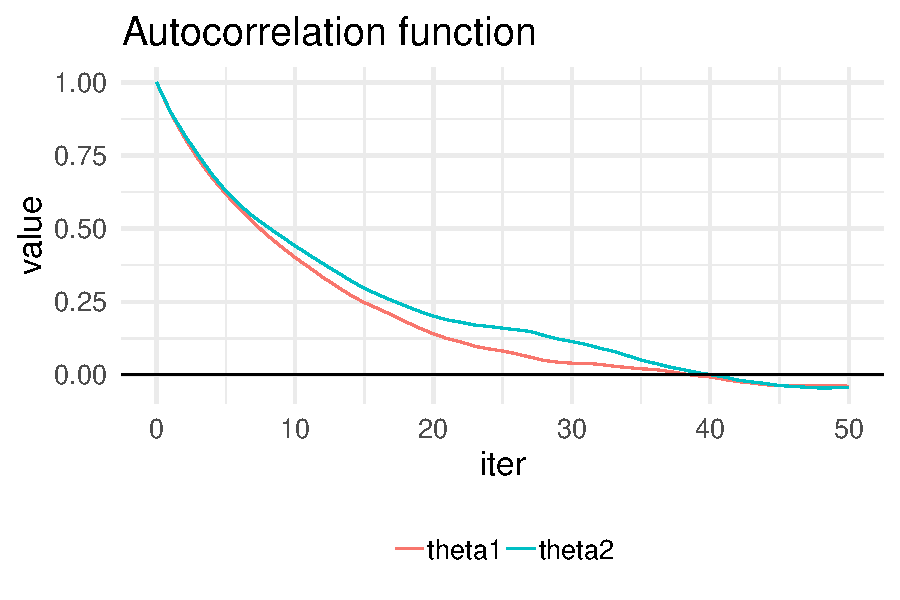
\includegraphics[width=7cm]{Metrop1acf.pdf}}
  
\end{frame}

\begin{frame}

  {\Large\color{navyblue} Auto correlation}

  \vspace{-0.5\baselineskip}
  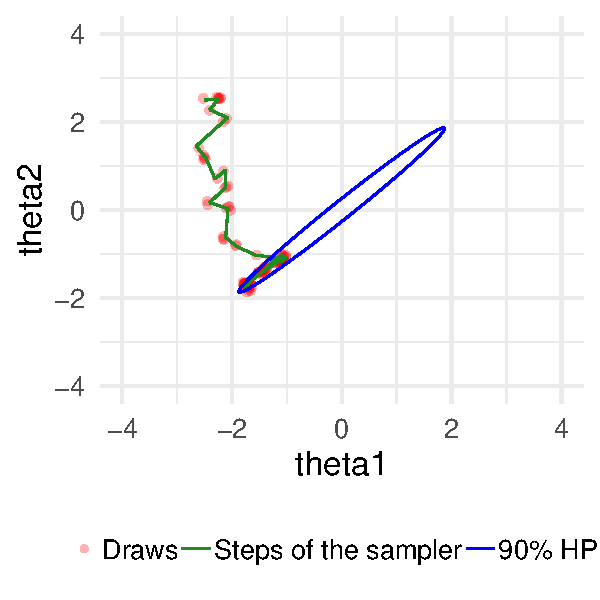
\includegraphics[width=4.5cm]{Metrop2.pdf}
  {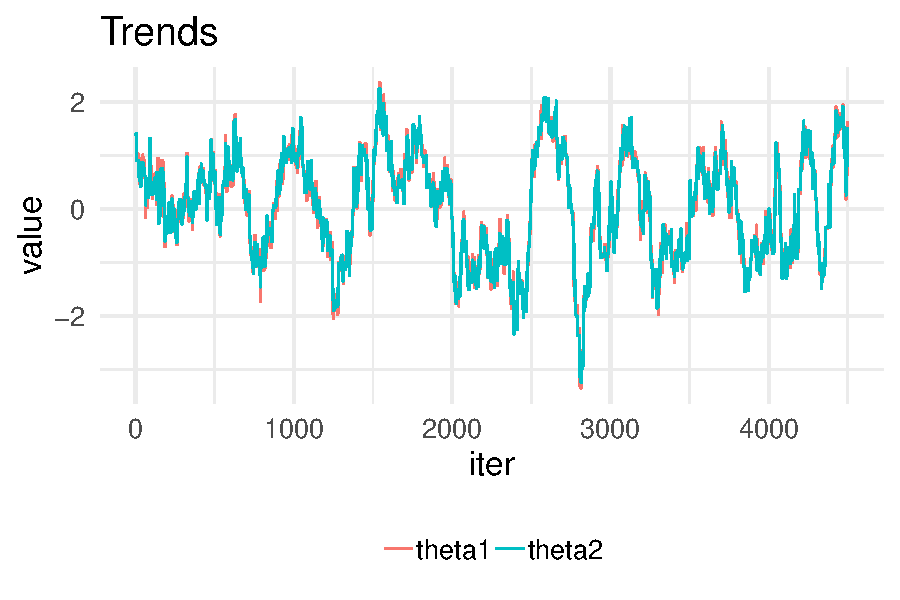
\includegraphics[width=7cm]{Metrop2trace.pdf}\\}
  {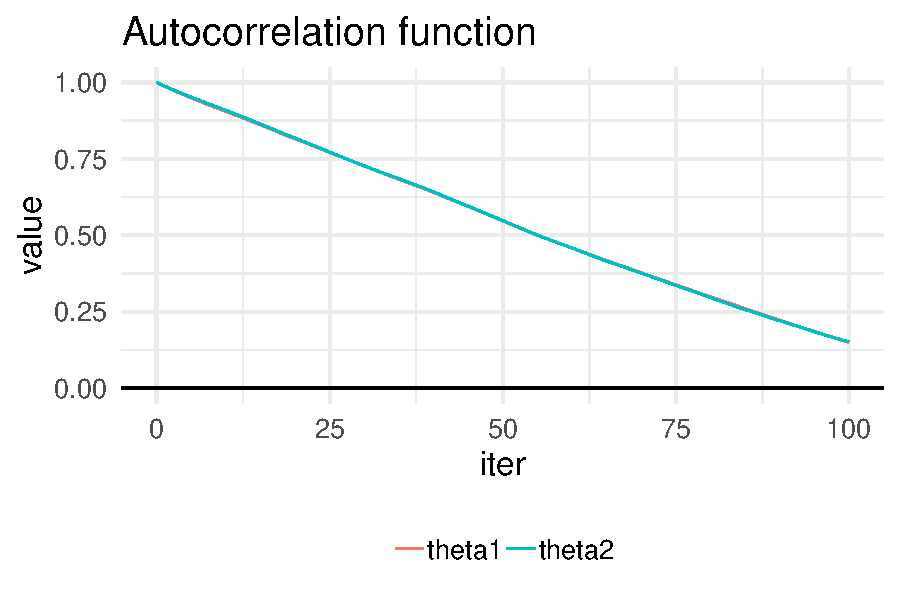
\includegraphics[width=7cm]{Metrop2acf.pdf}}
  
\end{frame}

\begin{frame}

  {\Large\color{navyblue} Auto correlation}

  \vspace{-0.5\baselineskip}
  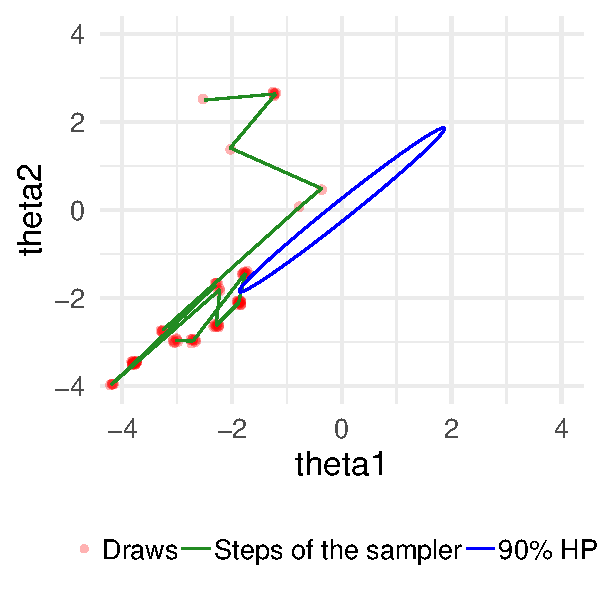
\includegraphics[width=4.5cm]{Metrop3.pdf}
  {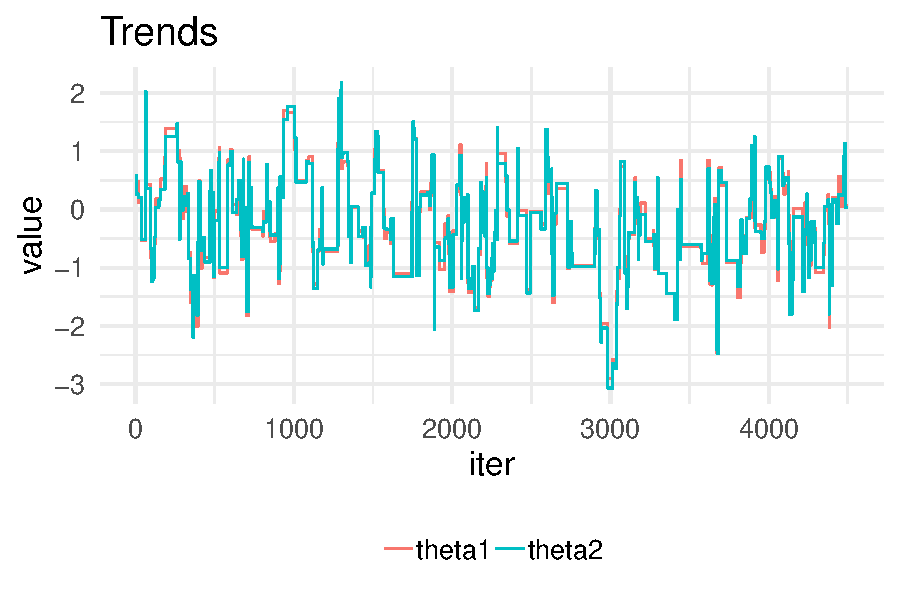
\includegraphics[width=7cm]{Metrop3trace.pdf}\\}
  {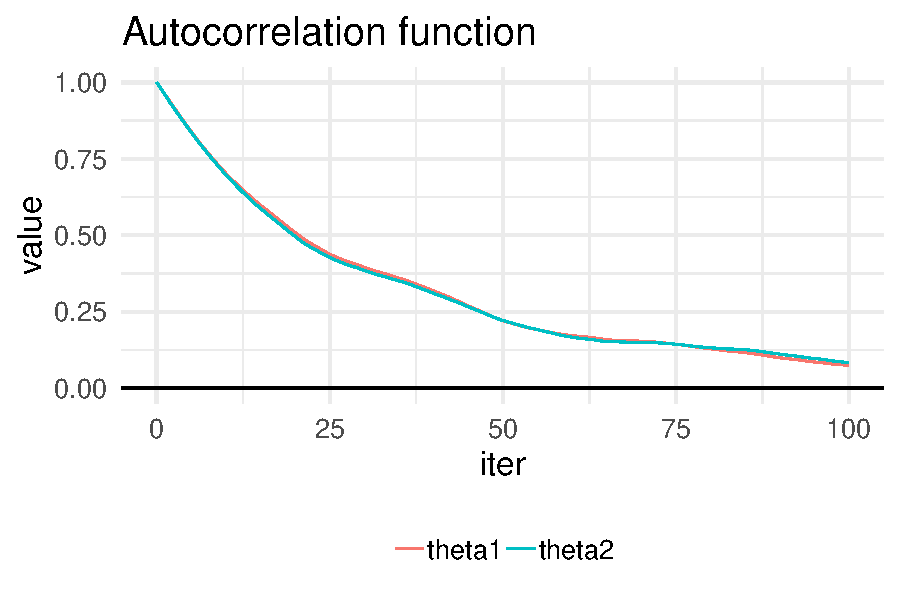
\includegraphics[width=7cm]{Metrop3acf.pdf}}
  
\end{frame}

\begin{frame}

  {\Large\color{navyblue} Time series analysis}

  \begin{itemize}
  \item Time series analysis can be used to estimate Monte Carlo
    error in case of MCMC
  \item For expectation $\bar{\theta}$
    \begin{equation*}
      \Var[\bar{\theta}] = \frac{\sigma^2_\theta}{N/\tau}
    \end{equation*}
    where $\tau$ is sum of autocorrelations
    \begin{itemize}
      \item $\tau$ describes how many dependent draws correspond to one independent sample
      \item in BDA3 $N=nm$
      \item $n_\eff=nm/\tau$
      \item BDA3 focuses on $n_\eff$ and not the Monte Carlo error directly
    \end{itemize}
  \end{itemize}  
\end{frame}

\begin{frame}

  {\Large\color{navyblue} Time series analysis}

  \begin{itemize}
  \item Estimation of the autocorrelation using several chains
    \begin{equation*}
      \hat{\rho}_t=1-\frac{W - \frac{1}{M}\sum_{j=1}^m \hat{\rho}_{t,j}}{2\widehat{\var}^{+}}
    \end{equation*}
    where $\hat{\rho}_{t,j}$ is autocorrelation at lag $t$ for chain $j$
  \item<2-> BDA3 has slightly different less accurate equation. The
    above equation is used in Stan 2.18+
  \item<3-> Compared to usual method which computes the autocorrelation
    from a single chain, this estimate has smaller variance
 \end{itemize}
\end{frame}

\begin{frame}

  {\Large\color{navyblue} Time series analysis}

  \begin{itemize}
  \item Estimation of $\tau$
    \begin{align*}
      \tau = 1 + 2 \sum_{t=1}^\infty \hat{\rho}_t
    \end{align*}
    where $\hat{\rho}_t$ is empirical autocorrelation 
    \begin{itemize}
    \item empirical autocorrelation function is noisy and thus
      estimate of $\tau$ is noisy
    \item noise is larger for longer lags (less observations)
    \item less noisy estimate is obtained by truncating
    \begin{align*}
      \tau \approx 1 + 2 \sum_{t=1}^T \hat{\rho}_t
    \end{align*}
    \end{itemize}
    \item<2-> As $\tau$ is estimated from a finite number of draws,
      it's expectation is overoptimistic
      \begin{itemize}
      \item if $\tau>mn/20$ then the estimate is unreliable

      \end{itemize} \end{itemize}
\end{frame}

\begin{frame}
  
  {\Large\color{navyblue} Geyer's adaptive window estimator}

  \begin{itemize}
  \item Truncation can be decided adaptively
    \begin{itemize}
    \item for stationary, irreducible, recurrent Markov chain
    \item let $\Gamma_m=\rho_{2m}+\rho_{2m+1}$, which is sum of two
      consequent autocorrelations
    \item $\Gamma_m$ is positive, decreasing and convex function of $m$
    \end{itemize}
    \vspace{0.5\baselineskip}
  \item<2-> Initial positive sequence estimator (Geyer's IPSE)
      \begin{itemize}
        \item Choose the largest $m$ so, that all values of the sequence
        $\hat{\Gamma}_1, \ldots, \hat{\Gamma}_m$ are positive
      \end{itemize}
  \vspace{0.5\baselineskip}
      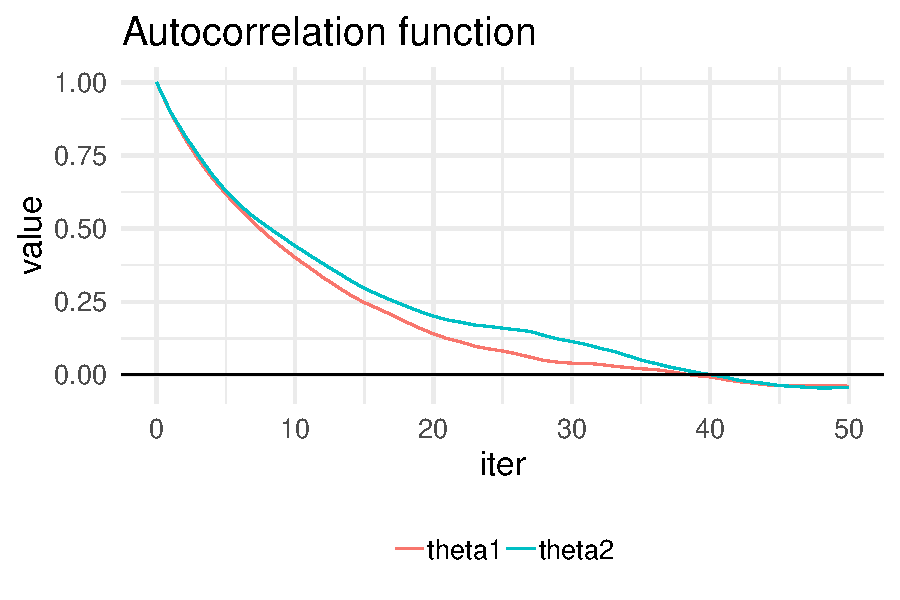
\includegraphics[width=6.5cm]{Metrop1acf.pdf}
  \end{itemize}
\end{frame}

% Gibbs1 neff=252, N=2001
% Gibbs2 neff=12, N=2001, Rhat 1.11
% Metrop1 neff=194, N=5000
% Metrop2 neff=48, N=5000
% Metrop3 neff=81, N=5000

\begin{frame}
  
   {\Large\color{navyblue} Effective sample size}

   Effective number of draws $n_\eff \approx N/\tau$\\
   \uncover<2->{
  \makebox[12cm][t]{
    \hspace{-.7cm}
     \begin{minipage}{12cm}
     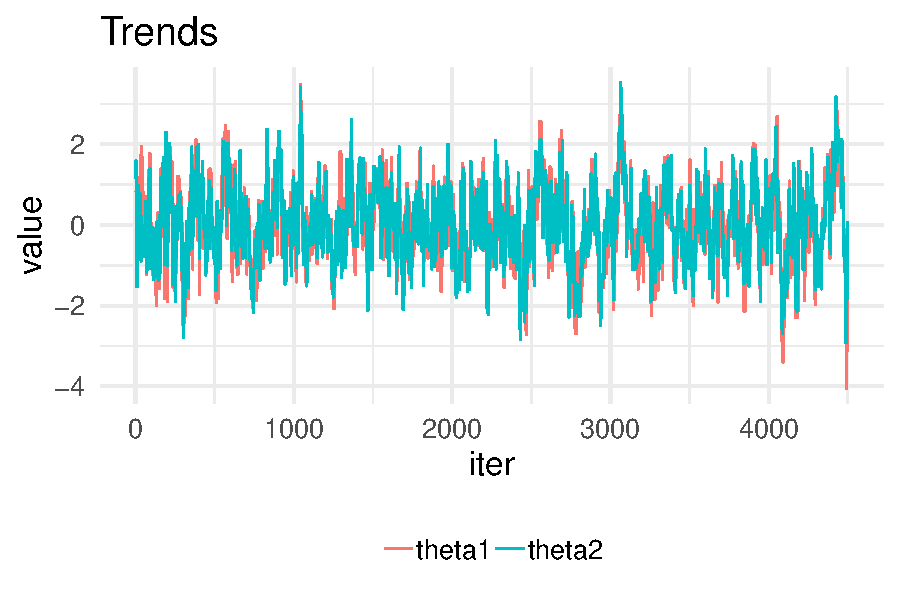
\includegraphics[width=6cm]{Metrop1trace.pdf}
     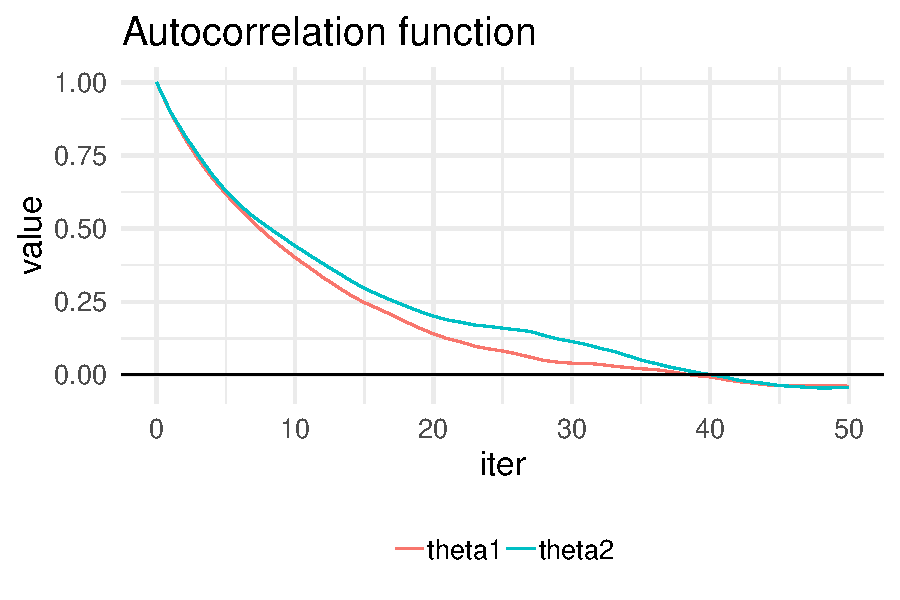
\includegraphics[width=6cm]{Metrop1acf.pdf}\\
     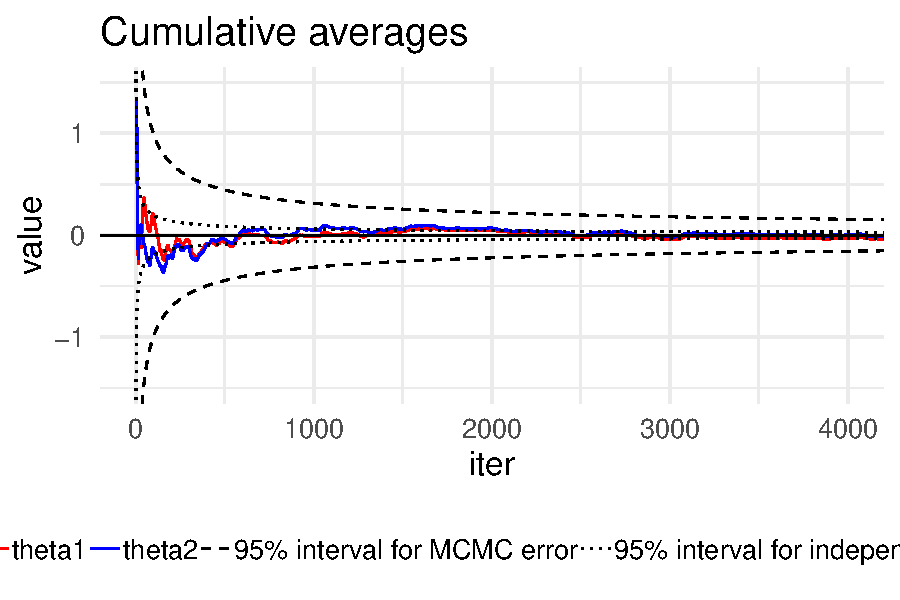
\includegraphics[width=6cm]{Metrop1mcerr.pdf}
     \hspace{0cm}
     \begin{minipage}[t][4cm][t]{6cm}
       \vspace{-3.5cm}
       \begin{align*}
         \tau & \approx 1 + 2 \sum_{t=1}^T \hat{\rho}_t\\
                 & \approx 24
       \end{align*}
     \end{minipage}
   \end{minipage}
   }
   }
   
\end{frame}

\begin{frame}
  
   {\Large\color{navyblue} Effective sample size}

   Effective number of draws $n_\eff \approx N/\tau$\\
  \makebox[12cm][t]{
    \hspace{-.7cm}
     \begin{minipage}{12cm}
     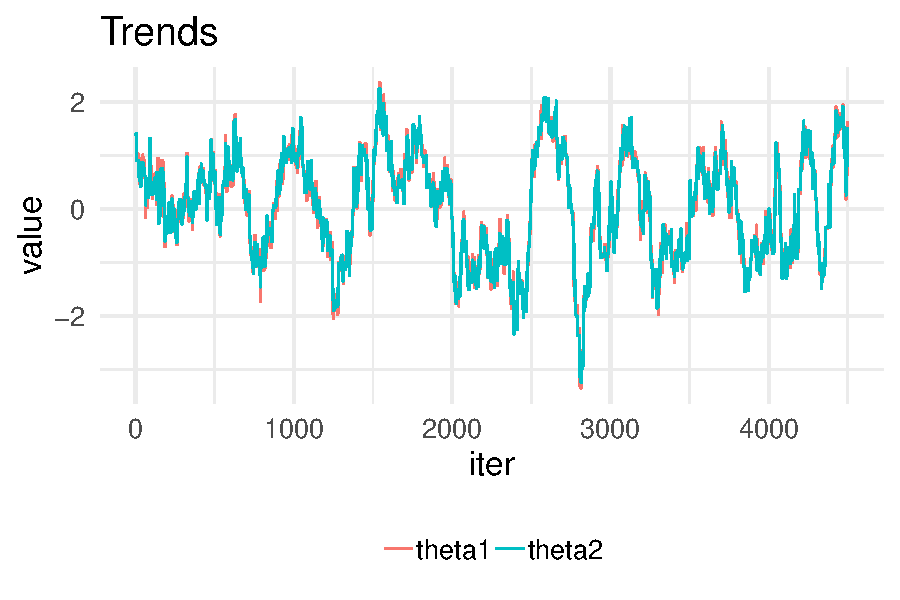
\includegraphics[width=6cm]{Metrop2trace.pdf}
     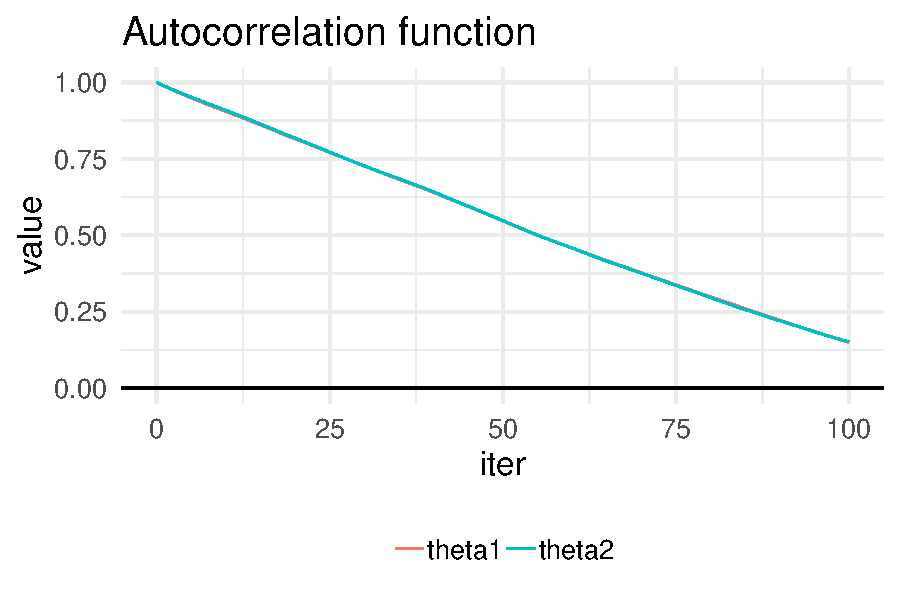
\includegraphics[width=6cm]{Metrop2acf.pdf}\\
     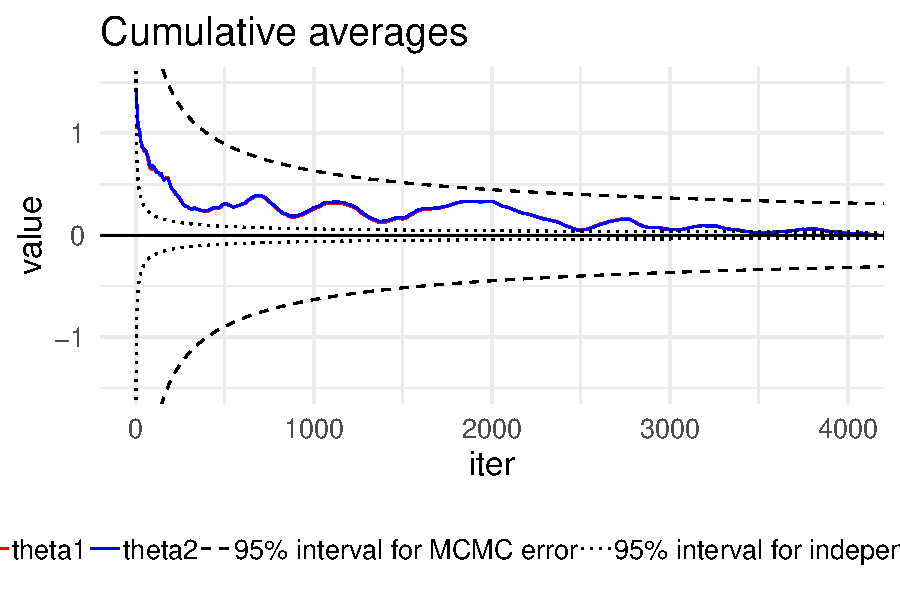
\includegraphics[width=6cm]{Metrop2mcerr.pdf}
     \hspace{0cm}
     \begin{minipage}[t][4cm][t]{6cm}
       \vspace{-3.5cm}
       \begin{align*}
         \tau & \approx 1 + 2 \sum_{t=1}^T \hat{\rho}_t\\
                 & \approx 104
       \end{align*}
     \end{minipage}
   \end{minipage}
   }
   
\end{frame}

\begin{frame}
  
   {\Large\color{navyblue} Effective sample size}

   Effective number of draws $n_\eff \approx N/\tau$\\
  \makebox[12cm][t]{
    \hspace{-.7cm}
     \begin{minipage}{12cm}
     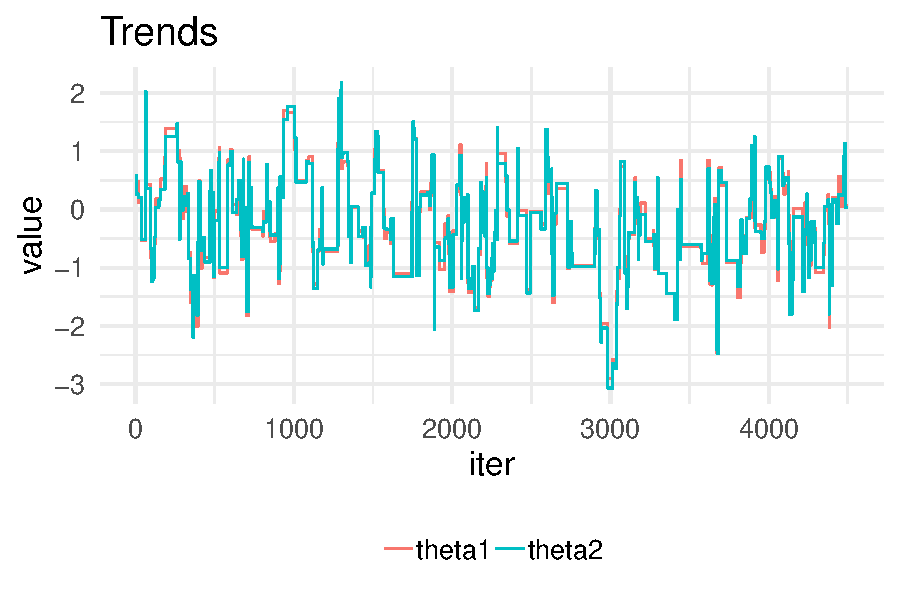
\includegraphics[width=6cm]{Metrop3trace.pdf}
     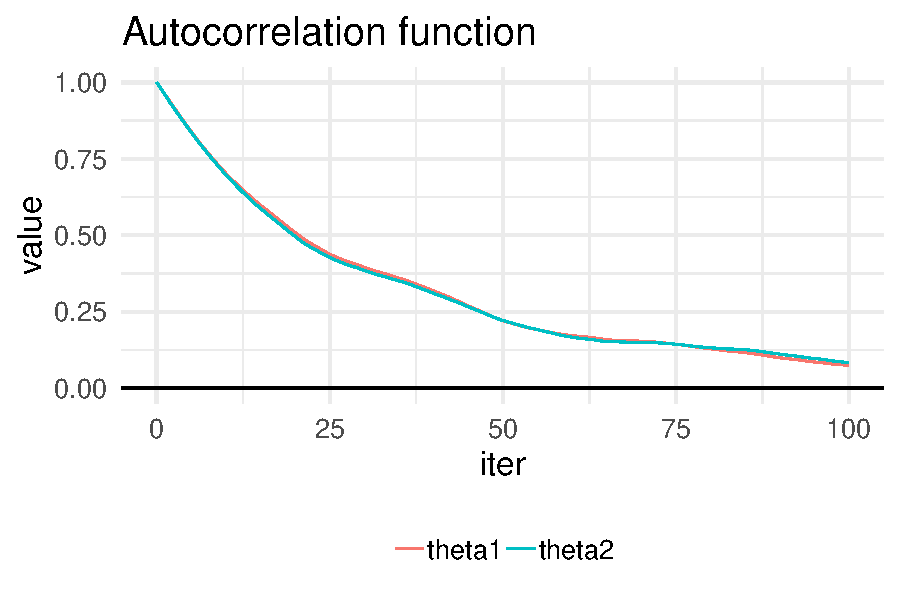
\includegraphics[width=6cm]{Metrop3acf.pdf}\\
     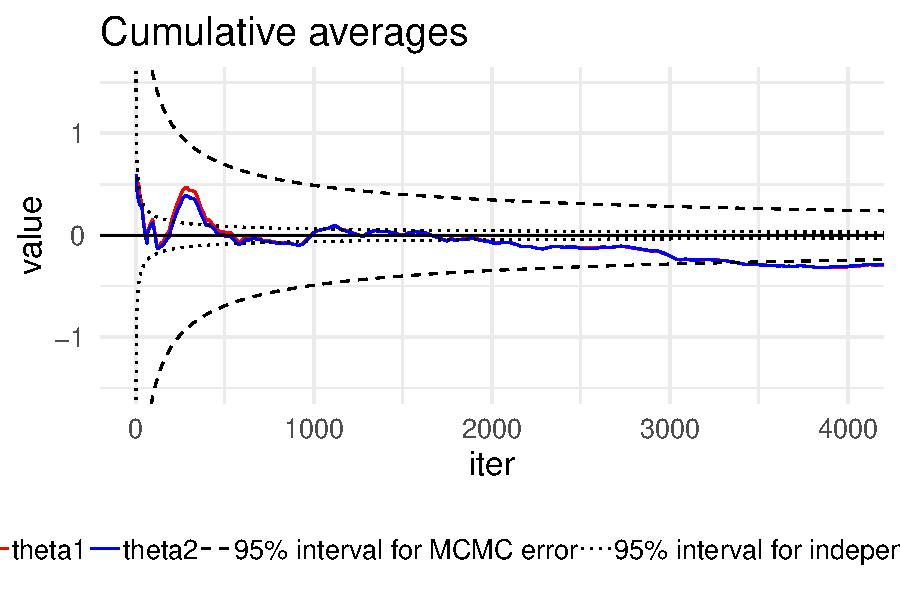
\includegraphics[width=6cm]{Metrop3mcerr.pdf}
     \hspace{0cm}
     \begin{minipage}[t][4cm][t]{6cm}
       \vspace{-3.5cm}
       \begin{align*}
         \tau & \approx 1 + 2 \sum_{t=1}^T \hat{\rho}_t\\
                 & \approx 63
       \end{align*}
     \end{minipage}
   \end{minipage}
   }
   
\end{frame}

\begin{frame}

  {\Large\color{navyblue} Problematic distributions}

  \begin{itemize}
  \item<1-> Nonlinear dependencies
    \begin{itemize}
    \item optimal proposal depends on location
    \end{itemize}
  \item<2-> Funnels
    \begin{itemize}
    \item optimal proposal depends on location
    \end{itemize}
  \item<3-> Multimodal
    \begin{itemize}
    \item difficult to move from one mode to another
    \end{itemize}
  \item<4-> Long-tailed with non-finite variance and mean
    \begin{itemize}
    \item central limit theorem for expectations does not hold
    \end{itemize}
  \end{itemize}

\end{frame}

\begin{frame}
  
   {\Large\color{navyblue} Next week: HMC, NUTS, and dynamic HMC}

   Effective number of draws $n_\eff \approx N/\tau$\\
  \makebox[12cm][t]{
    \hspace{-.7cm}
     \begin{minipage}{12cm}
     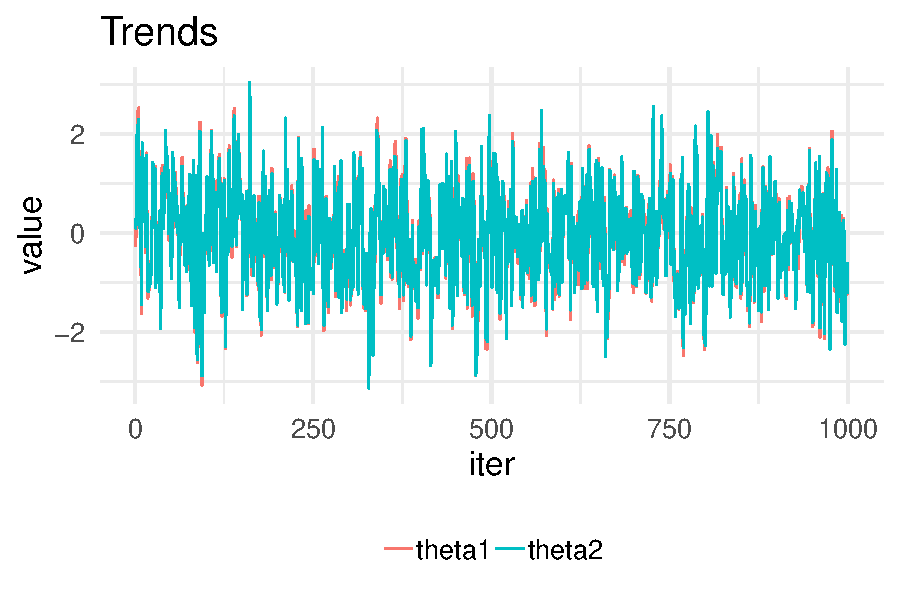
\includegraphics[width=6cm]{hmc1trace.pdf}
     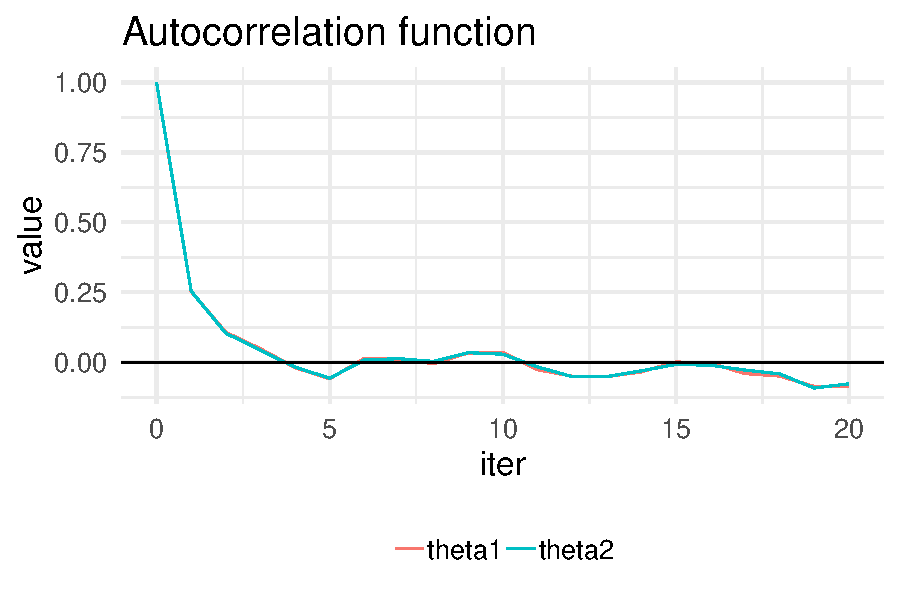
\includegraphics[width=6cm]{hmc1acf.pdf}\\
     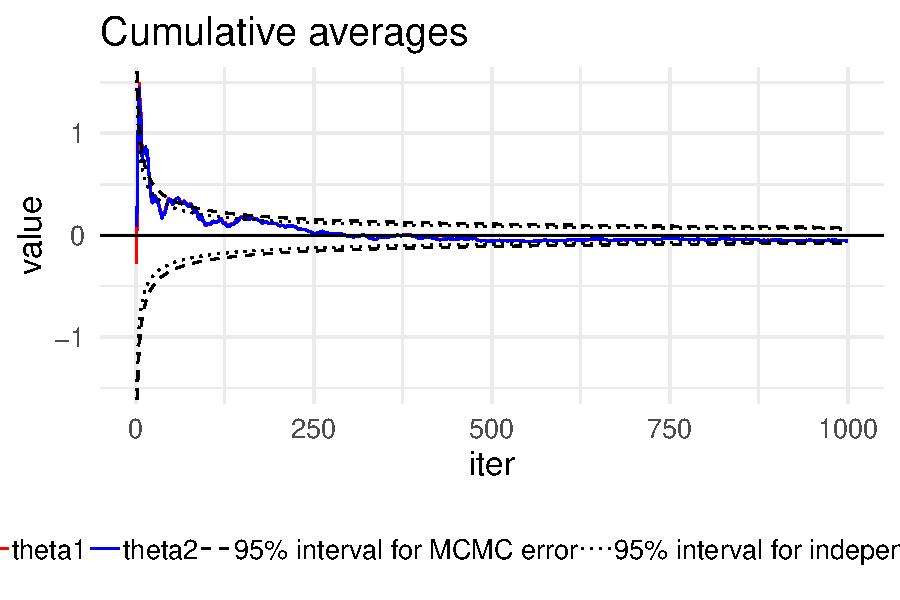
\includegraphics[width=6cm]{hmc1mcerr.pdf}
     \hspace{0cm}
     \begin{minipage}[t][4cm][t]{6cm}
       \vspace{-3.5cm}
       \begin{align*}
         \tau & \approx 1 + 2 \sum_{t=1}^T \hat{\rho}_t\\
                 & \approx 1.6
       \end{align*}
     \end{minipage}
   \end{minipage}
   }
   
\end{frame}

\begin{frame}
   
   {\Large\color{navyblue} Further diagnostics}

   \begin{itemize}
   \item Dynamic HMC/NUTS has additional diagnostics
     \begin{itemize}
     \item divergences
     \item tree depth exceedences
     \item fraction of missing information
     \end{itemize}
   \end{itemize}
   
 \end{frame}

\end{document}

%%% Local Variables: 
%%% TeX-PDF-mode: t
%%% TeX-master: t
%%% End: 
